\documentclass[11pt,a4paper,dvipsnames]{article}
\usepackage[margin=2.5cm]{geometry}
\usepackage{iohk}
\usepackage{microtype}
\usepackage{mathpazo} % nice fonts
\usepackage{amsmath}
\usepackage{amssymb}
\usepackage{amsthm}
\usepackage{latexsym}
\usepackage{mathtools}
\usepackage{stmaryrd}
\usepackage{extarrows}
\usepackage{slashed}
\usepackage[colon]{natbib}
\usepackage[unicode=true,pdftex,pdfa,colorlinks=true]{hyperref}
\usepackage{xcolor}
\usepackage[capitalise,noabbrev,nameinlink]{cleveref}
\usepackage{float}
\floatstyle{boxed}
\restylefloat{figure}

%%
%% Package `semantic` can be used for writing inference rules.
%%
\usepackage{semantic}
%% Setup for the semantic package
\setpremisesspace{20pt}

%%
%% Types
%%
\newcommand{\Tx}{\type{Tx}}
\newcommand{\Ix}{\type{Ix}}
\newcommand{\TxId}{\type{TxId}}
\newcommand{\Addr}{\type{Addr}}
\newcommand{\UTxO}{\type{UTxO}}
\newcommand{\Wdrl}{\type{Wdrl}}
\newcommand{\Value}{\type{Value}}
\newcommand{\Coin}{\type{Coin}}
\newcommand{\PrtclConsts}{\type{PrtclConsts}}
\newcommand{\Slot}{\type{Slot}}
\newcommand{\Duration}{\type{Duration}}
\newcommand{\Allocs}{\type{Allocs}}

\newcommand{\DCert}{\type{DCert}}
\newcommand{\DCertRegKey}{\type{DCert_{regkey}}}
\newcommand{\DCertDeRegKey}{\type{DCert_{deregkey}}}
\newcommand{\DCertDeleg}{\type{DCert_{delegate}}}
\newcommand{\DCertRegPool}{\type{DCert_{regpool}}}
\newcommand{\DCertRetirePool}{\type{DCert_{retirepool}}}
\newcommand{\StakePool}{\type{StakePool}}
\newcommand{\UTxOState}{\ensuremath{\type{UTxOState}}}
\newcommand{\ledgerState}{\ensuremath{\type{ledgerState}}}

\newcommand{\AddrRWD}{\type{Addr_{rwd}}}
\newcommand{\Ptr}{\type{Ptr}}
\newcommand{\DState}{\type{DState}}
\newcommand{\DWState}{\type{DWState}}
\newcommand{\DWEnv}{\type{DWEnv}}
\newcommand{\PState}{\type{PState}}
\newcommand{\DCertBody}{\type{DCertBody}}
\newcommand{\TData}{\type{TData}}
\newcommand{\DPoolReap}{\ensuremath{\type{poolreap}}}

%% Adding witnesses
\newcommand{\TxIn}{\type{TxIn}}
\newcommand{\TxOut}{\type{TxOut}}
\newcommand{\VKey}{\type{VKey}}
\newcommand{\SKey}{\type{SKey}}
\newcommand{\HashKey}{\type{HashKey}}
\newcommand{\KeyPair}{\type{KeyPair}}
\newcommand{\Sig}{\type{Sig}}
\newcommand{\Data}{\type{Data}}
%% Adding delegation
\newcommand{\Epoch}{\type{Epoch}}
\newcommand{\VKeyGen}{\type{VKeyGen}}
%% Blockchain
\newcommand{\Gkeys}{\var{G_{keys}}}
\newcommand{\Block}{\type{Block}}
\newcommand{\SlotId}{\type{SlotId}}
\newcommand{\UTxOEnv}{\type{UTxOEnv}}
\newcommand{\CEEnv}{\type{CEEnv}}
\newcommand{\CEState}{\type{CEState}}
\newcommand{\BDEnv}{\type{BDEnv}}
\newcommand{\BDState}{\type{BDState}}
\newcommand{\LEnv}{\type{LEnv}}
\newcommand{\LState}{\type{LState}}

%%
%% Functions
%%
\newcommand{\txins}[1]{\fun{txins}~ \var{#1}}
\newcommand{\txid}[1]{\fun{txid}~ \var{#1}}
\newcommand{\txouts}[1]{\fun{txouts}~ \var{#1}}
\newcommand{\values}[1]{\fun{values}~ #1}
\newcommand{\balance}[1]{\fun{balance}~ \var{#1}}
\newcommand{\ttl}[1]{\fun{ttl}~ \var{#1}}
\newcommand{\deposits}[2]{\fun{deposits}~ \var{#1} ~ \var{#2}}
\newcommand{\decayedKey}[4]{\fun{decayedKey}~ \var{#1}~ \var{#2}~ \var{#3}~ \var{#4}}
\newcommand{\decayedTx}[3]{\fun{decayedTx}~ \var{#1}~ \var{#2}~ \var{#3}}
\newcommand{\certRefund}[6]{\fun{certRefund}~ {#1}~{#2}~{#3}~\var{#4}~\var{#5}~\var{#6}}
\newcommand{\refund}[4]{\fun{refund}~ \var{#1}~ \var{#2}~ {#3}~ {#4}}
\newcommand{\keyRefunds}[3]{\fun{keyRefunds}~ \var{#1}~ \var{#2}~ \var{#3}}
\newcommand{\destroyed}[4]{\fun{destroyed}~ \var{#1}~ \var{#2}~ \var{#3}~ \var{#4}}
\newcommand{\created}[2]{\fun{created}~ \var{#1}~ \var{#2}}
\newcommand{\applyFun}[2]{\fun{#1}~\var{#2}}

\newcommand{\RegKey}[1]{\textsc{RegKey}(#1)}
\newcommand{\DeregKey}[1]{\textsc{DeregKey}(#1)}
\newcommand{\Delegate}[1]{\textsc{Delegate}(#1)}
\newcommand{\RegPool}[1]{\textsc{RegPool}(#1)}
\newcommand{\RetirePool}[1]{\textsc{RetirePool}(#1)}
\newcommand{\cauthor}[1]{\fun{author}~ \var{#1}}
\newcommand{\dpool}[1]{\fun{dpool}~ \var{#1}}
\newcommand{\stakepool}[1]{\fun{stakepool}~ \var{#1}}
\newcommand{\retire}[1]{\fun{retire}~ \var{#1}}
\newcommand{\addrRw}[1]{\fun{addr_{rwd}}~ \var{#1}}
\newcommand{\epoch}[1]{\fun{epoch}~ \var{#1}}
\newcommand{\dcerts}[1]{\fun{dcerts}~ \var{#1}}

%% UTxO witnesses
\newcommand{\inputs}[1]{\fun{inputs}~ \var{#1}}
\newcommand{\txwits}[1]{\fun{txwits}~ \var{#1}}
\newcommand{\verify}[3]{\fun{verify} ~ #1 ~ #2 ~ #3}
\newcommand{\sign}[2]{\fun{sign} ~ #1 ~ #2}
\newcommand{\serialised}[1]{\llbracket \var{#1} \rrbracket}
\newcommand{\addr}[1]{\fun{addr}~ \var{#1}}
\newcommand{\hashKey}[1]{\fun{hashKey}~ \var{#1}}
\newcommand{\txbody}[1]{\fun{txbody}~ \var{#1}}
\newcommand{\txdata}[1]{\fun{txdata}~ \var{#1}}
\newcommand{\txfee}[1]{\fun{txfee}~ \var{#1}}
\newcommand{\txwdrls}[1]{\fun{txwdrls}~ \var{#1}}
\newcommand{\minfee}[2]{\fun{minfee}~ \var{#1}~ \var{#2}}
\newcommand{\slotminus}[2]{\var{#1}~-_{s}~\var{#2}}
\DeclarePairedDelimiter\floor{\lfloor}{\rfloor}
% wildcard parameter
\newcommand{\wcard}[0]{\underline{\phantom{a}}}
%% Adding ledgers...
\newcommand{\utxo}[1]{\fun{utxo}~ #1}
%% Delegation
\newcommand{\delegatesName}{\fun{delegates}}
\newcommand{\delegates}[3]{\delegatesName~#1~#2~#3}
\newcommand{\dwho}[1]{\fun{dwho}~\var{#1}}
\newcommand{\depoch}[1]{\fun{depoch}~\var{#1}}
\newcommand{\dval}{\ensuremath{d_{\mathsf{val}}}}
%% Delegation witnesses
\newcommand{\dbody}[1]{\fun{dbody}~\var{#1}}
\newcommand{\dwit}[1]{\fun{dwit}~\var{#1}}
%% Blockchain
\newcommand{\bwit}[1]{\fun{bwit}~\var{#1}}
\newcommand{\bslot}[1]{\fun{bslot}~\var{#1}}
\newcommand{\bbody}[1]{\fun{bbody}~\var{#1}}
\newcommand{\bdlgs}[1]{\fun{bdlgs}~\var{#1}}
%% ledgerstate constants
\newcommand{\genesisId}{\ensuremath{Genesis_{Id}}}
\newcommand{\genesisTxOut}{\ensuremath{Genesis_{Out}}}
\newcommand{\genesisUTxO}{\ensuremath{Genesis_{UTxO}}}
\newcommand{\emax}{\ensuremath{\mathsf{E_{max}}}}
\newcommand{\slotsPer}{\ensuremath{\mathsf{slotsPerEpoch}}}

\theoremstyle{definition}
\newtheorem{definition}{Definition}[section]

\theoremstyle{definition}
\newtheorem{property}{Property}[section]

\begin{document}

\hypersetup{
  pdftitle={Formal Specification of the Cardano Ledger with a Native
  Multicurrency Implementation},
  breaklinks=true,
  bookmarks=true,
  colorlinks=false,
  linkcolor={blue},
  citecolor={blue},
  urlcolor={blue},
  linkbordercolor={white},
  citebordercolor={white},
  urlbordercolor={white}
}

\title{Formal Specification of the Cardano Ledger with a Native
Multicurrency Implementation}

\author{
   Polina Vinogradova \\ {\small \texttt{polina.vinogradova@iohk.io}} \\
   }

\date{}

\maketitle

\begin{abstract}
This document presents the modifications of the Shelley ledger
specification
(see~\cite{shelley_spec}) which will enable it to support native
Multicurrency (see~\cite{multi_currency} and~\cite{formal_multicur})
using a small scripting language fully specified
by the ledger rules.
\end{abstract}

\section*{List of Contributors}
\label{acknowledgements}

Duncan Coutts,
Philipp Kant,
Michal Peyton Jones,
Jann Mueller,
Jared Corduan,
Matthias Gudemann,
Manuel Chakravarty,
Kevin Hammond


\tableofcontents
\listoffigures

\section{Introduction}
\label{sec:introduction}
\section{Introduction}
\label{sec:introduction}

This specification models the \textit{conditions} that the different parts of a
transaction have to fulfill so that they can extend a ledger, which is
represented here as a list of transactions. In particular, we model the
following aspects:

\begin{description}
\item[Preservation of value] relationship between the total value of input and
  outputs in a new transaction, and the unspent outputs.
\item[Witnesses] authentication of parts of the transaction data by means of
  cryptographic entities (such as signatures and private keys) contained in
  these transactions.
\item[Delegation] validity of delegation certificates, which delegate
  block-signing rights.
\item[Update validation] voting mechanism which captures the identification of
  the voters, and the participants that can post update proposals.
\end{description}

The following aspects will not be modeled (since they are not part of the Byron
release):
\begin{description}
\item[Stake] staking rights associated to an addresses.
\end{description}


\section{Notation}\label{sec:notation}

The transition system is explained in \cite{small_step_semantics}.

\begin{description}
\item[Powerset] Given a set $\type{X}$, $\powerset{\type{X}}$ is the set of all
  the subsets of $X$.
\item[Symmetric Difference] Given two sets $\type{X}$ and $\type{Y}$,
  the symmetric difference of $\type{X}$ and $\type{Y}$,
  denoted $\type{X}\triangle\type{Y}$, is the union of $\type{X}$ and $\type{Y}$
  without the intersection.
\item[Sequences] Given a set $\type{X}$, $\seqof{\type{X}}$ is the set of
  sequences having elements taken from $\type{X}$. The empty sequence is
  denoted by $\epsilon$, and given a sequence $\Lambda$, $\Lambda; \type{x}$ is
  the sequence that results from appending $\type{x} \in \type{X}$ to
  $\Lambda$.
\item[Functions] $A \to B$ denotes a \textbf{total function} from $A$ to $B$.
  Given a function $f$ we write $f~a$ for the application of $f$ to argument
  $a$.
\item[Fibre] Given a function $f: A \to B$ and $b\in B$, we write
  $f^{-1}~b$ for the \textbf{fibre} of $f$ at $b$, which is defined by
  $\{a \mid\ f a =  b\}$.
\item[Maps and partial functions] $A \mapsto B$ denotes a \textbf{partial
    function} from $A$ to $B$, which can be seen as a map (dictionary) with
  keys in $A$ and values in $B$. Given a map $m \in A \mapsto B$, notation
  $a \mapsto b \in m$ is equivalent to $m~ a = b$.
\item[Map Operations] Figure \ref{fig:notation:nonstandard}
  describes some non-standard map operations.

\end{description}

In Figure~\ref{fig:notation:nonstandard}, we specify the notation we use in
the rest of the document.

\begin{figure}
  \begin{align*}
    \var{set} \restrictdom \var{map}
    & = \{ k \mapsto v \mid k \mapsto v \in \var{map}, ~ k \in \var{set} \}
    & \text{domain restriction}
    \\
    \var{set} \subtractdom \var{map}
    & = \{ k \mapsto v \mid k \mapsto v \in \var{map}, ~ k \notin \var{set} \}
    & \text{domain exclusion}
    \\
    \var{map} \restrictrange \var{set}
    & = \{ k \mapsto v \mid k \mapsto v \in \var{map}, ~ v \in \var{set} \}
    & \text{range restriction}
    \\
    \var{map} \subtractrange \var{set}
    & = \{ k \mapsto v \mid k \mapsto v \in \var{map}, ~ v \notin \var{set} \}
    & \text{range exclusion}
    \\
    M \unionoverrideRight N
    & = (\dom N \subtractdom M)\cup N
    & \text{union override right}
    \\
    M \unionoverrideLeft N
    & = M \cup (\dom M \subtractdom N)
    & \text{union override left}
    \\
    M \unionoverridePlus N
    & = (M \triangle N)
    \cup \{k\mapsto v_1+v_2\mid {k\mapsto v_1}\in M \land {k\mapsto v_2}\in N \}
    & \text{union override plus} \\
    & & \text{(for monoidal values)}\\
  \end{align*}
  \caption{Non-standard map operators}
  \label{fig:notation:nonstandard}
\end{figure}


\section{Cryptographic primitives}
\label{sec:crypto-primitives}


Figure~\ref{fig:crypto-defs} introduces the cryptographic abstractions used in
this document. We begin by listing the abstract types, which are meant to
represent the corresponding concepts in cryptography. Only the functionality
explicitly stated in the figures below is assumed within the scope of this paper.
That is, their exact
implementation remains open to interpretation, and we do not rely on
any additional properties derived from the study or implementation of public key
cryptography outside this work. The types and rules we give here are needed in
order to guarantee certain security properties of the delegation process, which
we discuss later.

The cryptographic concepts required for the formal definition
of witnessing include public-private key pairs, one-way functions
and signatures. The constraint we introduce states that a signature of
some data signed with a (private) key is only correct whenever we can verify
it using the corresponding public key.

\begin{figure}
  \emph{Abstract types}
  %
  \begin{equation*}
    \begin{array}{r@{~\in~}lr}
      \var{sk} & \SKey & \text{private signing key}\\
      \var{vk} & \VKey & \text{public verifying key}\\
      \var{hk} & \HashKey & \text{hashKey of a key}\\
      \sigma & \Sig  & \text{signature}\\
      \var{d} & \Data  & \text{data}\\
    \end{array}
  \end{equation*}
  \emph{Derived types}
  \begin{equation*}
    \begin{array}{r@{~\in~}lr}
      (sk, vk) & \KeyPair & \text{signing-verifying key pairs}
    \end{array}
  \end{equation*}
  \emph{Abstract functions}
  %
  \begin{equation*}
    \begin{array}{r@{~\in~}lr}
      \hashKey{} & \VKey \to \HashKey
      & \text{hashKey function} \\
      %
      \fun{verify} & \powerset{\left(\VKey \times \Data \times \Sig\right)}
      & \text{verification relation}\\
    \end{array}
  \end{equation*}
  \emph{Constraints}
  \begin{align*}
    & \forall (sk, vk) \in \KeyPair,~ m \in \Data,~ \sigma \in \Sig \cdot
      \verify{vk}{m}{\sigma} \iff \sign{sk}{m} = \sigma
  \end{align*}
  \emph{Notation for serialized and verified data}
  \begin{align*}
    & \serialised{x} & \text{serialised representation of } x\\
    & \mathcal{V}_{\var{vk}}{\serialised{m}}_{\sigma} = \verify{vk}{m}{\sigma}
      & \text{shorthand notation for } \fun{verify}
  \end{align*}
  \caption{Cryptographic definitions}
  \label{fig:crypto-defs}
\end{figure}

\clearpage

\section{Serialization}
\label{sec:serialization}


Besides basic cryptographic abstractions, we also make use of some abstract
data storage properties in this document in order to build necessary definitions
and make judgement calls about them.

Abstract data types in this paper are essentially placeholders with names
indicating the data types they are meant to represent in an implementation.
Derived types are made up of data structures (i.e. products, lists, finite
maps, etc.) built from abstract types. The underlying structure of a data type
is implementation-dependent, and furthermore, the way the data is stored on
physical storage can vary as well.

Serialization is a physical manipulation of data on a given storage device.
In this document, the properties and rules we state involving serialization are
assumed to hold true independently of the storage medium and style of data
organization chosen for an implementation.

\section{Delegation}
\label{sec:delegation}
\section{Delegation}
\label{sec:delegation}

An agent owning a key that can sign new blocks can delegate its signing rights
to another key by means of \textit{delegation certificates}. These certificates
are included in the ledger, and therefore also included in the body of the
blocks in the blockchain.

There are several restrictions on a certificate posted on the blockchain:
\begin{enumerate}
\item Only genesis keys can delegate.
\item Certificates must be properly signed by the delegator.
\item Any given key can delegate at most once per-epoch.
\item Any given key can issue at most one certificate in a given slot.
\item The epochs in the certificates must refer to the current or to the next
  epoch. We do not want to allow certificates from past epochs so that a
  delegation certificate cannot be replayed. On the other hand if we allow
  certificates with arbitrary future epochs, then a malicious key can issue a
  delegation certificate per-slot, setting the epoch to a sufficiently large
  value. This will cause a blow up in the size of the ledger state since we
  will not be able to clean $\var{eks}$ (we only clean past epochs). Also note
  that we do not check the relation between the certificate epoch and the slot
  in which the certificate becomes active. This would bring additional
  complexity without any obvious benefit.
\item Certificates do not become active immediately, but they require a certain
  number of slots till they become stable in all the nodes.
\end{enumerate}
These conditions are formalized in \cref{fig:rules:delegation-scheduling}.
Rule~\ref{eq:rule:delegation-scheduling} determines when a certificate can
become ``scheduled''. The definitions used in this rules are presented in
\cref{fig:defs:delegation-scheduling}, and the types of the system induced by
$\trans{sdeleg}{\wcard}$ are presented in
\cref{fig:ts-types:delegation-scheduling}.

\begin{figure}[htb]
  \emph{Abstract types}
  \begin{equation*}
    \begin{array}{r@{~\in~}lr}
      c & \DCert & \text{delegation certificate}\\
      \var{vk_g} & \VKeyGen & \text{genesis verification key}\\
    \end{array}
  \end{equation*}

  \emph{Derived types}
  \begin{equation*}
    \begin{array}{r@{~\in~}l@{\qquad=\qquad}r@{~\in~}lr}
      \var{e} & \Epoch & n & \mathbb{N} & \text{epoch}\\
      \var{s} & \Slot & s & \mathbb{N} & \text{slot}\\
      \var{d} & \SlotCount & s & \mathbb{N} & \text{slot}
    \end{array}
  \end{equation*}

  \emph{Constraints}
  \begin{align*}
    \VKeyGen \subseteq \VKey
  \end{align*}

  \emph{Abstract functions}
  \begin{equation*}
    \begin{array}{r@{~\in~}lr}
      \fun{dbody} & \DCert \to (\VKey \times \Epoch)
      & \text{body of the delegation certificate}\\
      \fun{dwit} & \DCert \to (\VKeyGen \times \Sig)
      & \text{witness for the delegation certificate}\\
      \fun{dwho} & \DCert \mapsto (\VKeyGen \times \VKey)
      & \text{who delegates to whom in the certificate}\\
      \fun{depoch} & \DCert \mapsto \Epoch
      & \text{certificate epoch}
    \end{array}
  \end{equation*}
  \caption{Delegation scheduling definitions}
  \label{fig:defs:delegation-scheduling}
\end{figure}

\begin{figure}[htb]
  \emph{Delegation scheduling environments}
  \begin{equation*}
    \DSEnv =
    \left(
      \begin{array}{r@{~\in~}lr}
        \mathcal{K} & \powerset{\VKeyGen} & \text{allowed delegators}\\
        \var{e} & \Epoch & \text{epoch}\\
        \var{s} & \Slot & \text{slot}\\
        \var{k} & \SlotCount & \text{chain stability parameter}
      \end{array}
    \right)
  \end{equation*}

  \emph{Delegation scheduling states}
  \begin{equation*}
    \DSState
    = \left(
      \begin{array}{r@{~\in~}lr}
        \var{sds} & \seqof{(\Slot \times (\VKeyGen \times \VKey))} & \text{scheduled delegations}\\
        \var{eks} & \powerset{(\Epoch \times \VKeyGen)} & \text{key-epoch delegations}
      \end{array}
    \right)
  \end{equation*}

  \emph{Delegation scheduling transitions}
  \begin{equation*}
    \var{\_} \vdash
    \var{\_} \trans{sdeleg}{\_} \var{\_}
    \subseteq \powerset (\DSEnv \times \DSState \times \DCert \times \DSState)
  \end{equation*}
  \caption{Delegation scheduling transition-system types}
  \label{fig:ts-types:delegation-scheduling}
\end{figure}

\begin{figure}[htb]
  \begin{equation}
    \inference
    {
    }
    {
      {\begin{array}{l}
       \mathcal{K}\\
        e\\
        s\\
        d
      \end{array}}
      \vdash
      \left(
        \begin{array}{l}
          \epsilon\\
          \emptyset
        \end{array}
      \right)
    }
  \end{equation}
  \nextdef
  \begin{equation}
    \label{eq:rule:delegation-scheduling}
    \inference
    {
      (\var{vk_s},~ \sigma) \leteq \dwit{c}
      & \verify{vk_s}{\serialised{\dbody{c}}}{\sigma} & vk_s \in \mathcal{K}\\ ~ \\
      (\var{vk_s},~ \var{vk_d}) \leteq \dwho{c} & e_d \leteq \depoch{c}
      & (e_d,~ \var{vk_s}) \notin \var{eks} & 0 \leq e_d - e \leq 1 \\ ~ \\
      d \leteq 2 \cdot k & (s + d,~ (\var{vk_s},~ \wcard)) \notin \var{sds}\\
    }
    {
      {\begin{array}{l}
       \mathcal{K}\\
        e\\
        s\\
        k
      \end{array}}
      \vdash
      {
        \left(
          \begin{array}{l}
            \var{sds}\\
            \var{eks}
          \end{array}
        \right)
      }
      \trans{sdeleg}{c}
      {
        \left(
          \begin{array}{l}
            \var{sds}; (s + d,~ (\var{vk_s},~ \var{vk_d}))\\
            \var{eks} \cup \{(e_d,~ \var{vk_s})\}
          \end{array}
        \right)
      }
    }
  \end{equation}
  \caption{Delegation scheduling rules}
  \label{fig:rules:delegation-scheduling}
\end{figure}

\clearpage

The rules in Figure~\ref{fig:rules:delegation} model the activation of
delegation certificates. Once a scheduled certificate becomes active
(see~\cref{sec:delegation-interface-rules}), the delegation map is changed by
it only if:
\begin{itemize}
\item The delegating key ($\var{vk_s}$) did not activate a delegation
  certificate in a slot greater or equal than the certificate slot ($s$). This
  check is performed to avoid having the constraint that the delegation
  certificates have to be activated in slot order.
\item The key being delegated to ($\var{vk_d}$) has not been delegated by
  another key (injectivity constraint).
\end{itemize}
The reason why we check that the delegation map is injective is to avoid a
potential risk (during the OBFT era) in which a malicious node gets control of
a genesis key $\var{vk_m}$ that issued the maximum number of blocks in a given
window. By delegating to another key $\var{vk_d}$, which was already delegated to
by some other key $\var{vk_g}$, the malicious node could prevent $\var{vk_g}$
from issuing blocks. Even though the delegation certificates take several slots
to become effective, the malicious node could calculate when the certificate
would become active, and issue a delegation certificate at the right time.

As an additional advantage, by having an injective delegation map, we are able
to simplify our specification when it comes to counting the blocks issued by
(delegates of) genesis keys.

Note also, that we could not impose the injectivity constraint in
Rule~\ref{eq:rule:delegation-scheduling} since we do not have information about
the delegations that will become effective. We could of course detect a
violation in the injectivity constraint when scheduling a delegation
certificate, but this will lead to a complex computation and larger state in
said rule.

Finally, note that we do not want to reject a scheduled delegation that would
violate the injectivity constraint (since delegation might not have been
scheduled by the node issuing the block). Instead, we simply ignore the
delegation certificate (Rule~\ref{eq:rule:delegation-nop}).

\begin{figure}[htb]
  \begin{align*}
    & \unionoverrideRight \in (A \mapsto B) \to (A \mapsto B) \to (A \mapsto B)
    & \text{union override}\\
    & d_0 \unionoverrideRight d_1 = d_1 \cup (\dom d_1 \subtractdom d_0)
  \end{align*}
  \caption{Functions used in delegation rules}
  \label{fig:funcs:delegation}
\end{figure}

\begin{figure}[htb]
  \emph{Delegation environments}
  \begin{equation*}
    \DEnv =
    \left(
      \begin{array}{r@{~\in~}lr}
        \mathcal{K} & \powerset{\VKeyGen} & \text{allowed delegators}
      \end{array}
    \right)
  \end{equation*}

  \emph{Delegation states}
  \begin{align*}
    & \DState
      = \left(
        \begin{array}{r@{~\in~}lr}
          \var{dms} & \VKeyGen \mapsto \VKey & \text{delegation map}\\
          \var{dws} & \VKeyGen \mapsto \Slot & \text{when last delegation occurred}\\
        \end{array}\right)
  \end{align*}
  \emph{Delegation transitions}
  \begin{equation*}
    \_ \vdash \_ \trans{adeleg}{\_} \_ \in
    \powerset (\DEnv \times \DState \times (\Slot \times (\VKeyGen \times \VKey)) \times \DState)
    \end{equation*}
  \caption{Delegation transition-system types}
  \label{fig:ts-types:delegation}
\end{figure}

\begin{figure}[htb]
  \begin{equation}
    \inference
    {
      \var{dms_0} \leteq \Set{k \mapsto k}{k \in \mathcal{K}} &
      \var{dws_0} \leteq \Set{k \mapsto 0}{k \in \mathcal{K}}
    }
    {
      \mathcal{K}
      \vdash
      \left(
        \begin{array}{l}
          \var{dms_0}\\
          \var{dws_0}
        \end{array}
      \right)
    }
  \end{equation}
  \nextdef
  \begin{equation}\label{eq:rule:delegation-change}
    \inference
    {
      \var{vk_d} \notin \range~\var{dms} & (\var{vk_s} \mapsto s_p \in \var{dws} \Rightarrow s_p < s)
    }
    {
      \mathcal{K}
      \vdash
      \left(
      \begin{array}{r}
        \var{dms}\\
        \var{dws}
      \end{array}
      \right)
      \trans{adeleg}{(s,~ (vk_s,~ vk_d))}
      \left(
      \begin{array}{lcl}
        \var{dms} & \unionoverrideRight & \{\var{vk_s} \mapsto \var{vk_d}\}\\
        \var{dws} & \unionoverrideRight & \{\var{vk_s} \mapsto s \}
      \end{array}
      \right)
    }
  \end{equation}
  \nextdef
  \begin{equation}\label{eq:rule:delegation-nop}
    \inference
    {\var{vk_d} \in \range~\var{dms} \vee (\var{vk_s} \mapsto s_p  \in \var{dws}  \wedge s \leq s_p)
    }
    {
      \mathcal{K}
      \vdash
      \left(
      \begin{array}{r}
        \var{dms}\\
        \var{dws}
      \end{array}
      \right)
      \trans{adeleg}{(s,~ (\var{vk_s},~ \var{vk_d}))}
      \left(
      \begin{array}{lcl}
        \var{dms}\\
        \var{dws}
      \end{array}
      \right)
    }
  \end{equation}
  \caption{Delegation inference rules}
  \label{fig:rules:delegation}
\end{figure}

\clearpage

\subsection{Delegation sequences}
\label{sec:delegation-sequences}

This section presents the rules that model the effect that sequences of
delegations have on the ledger.

\begin{figure}[htb]
  \begin{equation}
    \inference[Initial-SDELEGS]
    {
    }
    {
      {\begin{array}{l}
       \mathcal{K}\\
        e\\
        s\\
        d
      \end{array}}
      \vdash
      \left(
        \begin{array}{l}
          \epsilon\\
          \emptyset
        \end{array}
      \right)
    }
  \end{equation}
  \nextdef
  \begin{equation}
    \label{eq:rule:delegation-scheduling-seq-base}
    \inference
    {
    }
    {
      {\begin{array}{l}
         \mathcal{K} \\
         e\\
         s\\
         d
       \end{array}}
      \vdash
      {
        \left(
          \begin{array}{l}
            \var{sds}\\
            \var{eks}
          \end{array}
        \right)
      }
      \trans{sdelegs}{\epsilon}
      {
        \left(
          \begin{array}{l}
            \var{sds}\\
            \var{eks}
          \end{array}
        \right)
      }
    }
  \end{equation}
  \nextdef
  \begin{equation}
    \label{eq:rule:delegation-scheduling-seq-ind}
    \inference
    {
      {\begin{array}{l}
         \mathcal{K} \\
         e\\
         s\\
         d
       \end{array}}
      \vdash
      {
        \left(
          \begin{array}{l}
            \var{sds}\\
            \var{eks}
          \end{array}
        \right)
      }
      \trans{sdelegs}{\Gamma}
      {
        \left(
          \begin{array}{l}
            \var{sds'}\\
            \var{eks'}
          \end{array}
        \right)
      }
      &
      {\begin{array}{l}
         \mathcal{K} \\
         e\\
         s\\
         d
       \end{array}}
      \vdash
      {
        \left(
          \begin{array}{l}
            \var{sds'}\\
            \var{eks'}
          \end{array}
        \right)
      }
      \trans{sdeleg}{c}
      {
        \left(
          \begin{array}{l}
            \var{sds''}\\
            \var{eks''}
          \end{array}
        \right)
      }
    }
    {
      {\begin{array}{l}
         \mathcal{K} \\
         e\\
         s\\
         d
       \end{array}}
      \vdash
      {
        \left(
          \begin{array}{l}
            \var{sds}\\
            \var{eks}
          \end{array}
        \right)
      }
      \trans{sdelegs}{\Gamma; c}
      {
        \left(
          \begin{array}{l}
            \var{sds''}\\
            \var{eks''}
          \end{array}
        \right)
      }
    }
  \end{equation}
  \caption{Delegation scheduling sequence rules}
  \label{fig:rules:delegation-scheduling-seq}
\end{figure}

\begin{figure}
  \begin{equation}
    \inference[Initial-ADELEGS]
    {
      \var{dms_0} \leteq \Set{k \mapsto k}{k \in \mathcal{K}} &
      \var{dws_0} \leteq \Set{k \mapsto 0}{k \in \mathcal{K}}
    }
    {
      \mathcal{K}
      \vdash
      \left(
        \begin{array}{l}
          \var{dms_0}\\
          \var{dws_0}
        \end{array}
      \right)
    }
  \end{equation}
  \nextdef
  \begin{equation}
    \label{eq:rule:delegation-seq-base}
    \inference
    {
    }
    {
      \mathcal{K}
      \vdash
      {
        \left(
          \begin{array}{l}
            \var{dms}\\
            \var{dws}
          \end{array}
        \right)
      }
      \trans{adelegs}{\epsilon}
      {
        \left(
          \begin{array}{l}
            \var{dms}\\
            \var{dws}
          \end{array}
        \right)
      }
    }
  \end{equation}
  \nextdef
  \begin{equation}
    \label{eq:rule:delegation-seq-ind}
    \inference
    {
      {
        \left(
          \begin{array}{l}
            \var{dms}\\
            \var{dws}
          \end{array}
        \right)
      }
      \trans{adelegs}{\Gamma}
      {
        \left(
          \begin{array}{l}
            \var{dms'}\\
            \var{dws'}
          \end{array}
        \right)
      }
      &
      {
        \left(
          \begin{array}{l}
            \var{dms'}\\
            \var{dws'}
          \end{array}
        \right)
      }
      \trans{adeleg}{c}
      {
        \left(
          \begin{array}{l}
            \var{dms''}\\
            \var{dws''}
          \end{array}
        \right)
      }
    }
    {
      \mathcal{K}
      \vdash
      {
        \left(
          \begin{array}{l}
            \var{dms}\\
            \var{dws}
          \end{array}
        \right)
      }
      \trans{adelegs}{\Gamma; c}
      {
        \left(
          \begin{array}{l}
            \var{dms''}\\
            \var{dws''}
          \end{array}
        \right)
      }
    }
  \end{equation}
  \caption{Delegations sequence rules }
  \label{fig:rules:delegation-seq}
\end{figure}


\clearpage

\section{UTxO}
\label{sec:utxo}

A key constraint that must always be satisfied as a result and precondition of
a valid ledger state transition is called the \textit{general accounting
property}, or the \textit{preservation of value} condition. Every piece of
software that is a part of the implementation of the
Cardano cryptocurrency must function in such a way as to not result in
a violation of this rule.
If this condition is not satisfied, it is an indicator of
incorrect accounting, potentially due to
malicious disruption or a bug.

The preservation of value is expressed as an equality that uses values in
the ledger state and the environment, as well as the values in the body of
the signal transaction.
We have defined the rules of the delegation protocol in a way that should
consistently satisfy the preservation of value. In the future, we hope to
give a formally-verified proof that every \textit{valid} ledger state satisfies
this property.

In this section, we discuss the relevant accounting that needs to be done
as a result of processing a transaction, i.e. the deposits for all certificates,
transaction fees, transaction withdrawals, and refunds for individual
deregistration, so that we may keep track of whether the preservation of
value is satisfied. Stake pool retirement refunds are not triggered by a
transaction (but rather, happen at the epoch boundary), and are therefore
not considered in our state change rules invoked due to a signal transaction.

Note, that when a transaction is issued by a wallet to be applied to the ledger
state (i.e. processed),
we define the rules in this section in such a way that it is impossible to
apply only some parts of a transaction (e.g. only certain certificates).
Every part of the transaction must be valid and it must be live, otherwise
it is ignored entirely. It is the wallet's responsibility to inform the user
that a transaction failed to be processed.

\subsection{Deposits and Refunds}
\label{sec:deps-refunds}

We present the types of variables and functions needed for deposit and
refund calculations in Figure~\ref{fig:defs:deposits}.

The $\PrtclConsts$ is
an abstract type that will represent an environment variable that contains
values on which the functionality of the blockchain protocol depends, such
as the fees transactions are obligated to pay to be processed. In particular,
we define two maps here that return values stored in the set of protocol
constants. The map $\fun{dvalue}$ returns the amount a certificate must
deposit to claim a specific resource (i.e. for the declaration of a new staking
key or the registration of a stake pool, depending on the type of certificate).

The map $\fun{decay}$
represents the rate of decrease of the value of a unit of $\Coin$.
The constant returned by $\fun{decay}$ consists of two values. The first is
a natural number which determines the minimal proportion of a deposit that will
be refunded on resource release. The second is a positive rational number
used to determine the rate of (exponential) decrease of the value.
Recall that the $\Allocs$ type pairs a hash key with a slot number and is a generic datatype
which we use below to represent both individual and pool allocation
parameters passed to refund calculations.

For a given transaction and protocol constants, the map $\fun{dresource}$
returns all the certificates of that transaction which allocate resources
(i.e. the stake key and stake pool registration certificates). The map
$\fun{dderegister}$ returns the resource release certificates for the
deregistration of a stake key. The map which returns only
the retirement type certificates is $\fun{dretire}$. The function $\fun{ttl}$ gives the
time slot in which the validity of a given transaction will expire. That is,
after slot number $\fun{ttl}~\var{tx}$, the transaction will not be processed.
This value is generated by the wallet.

The functions used in refund calculations are presented in
Figure~\ref{fig:functions:deposits-refunds}.
The function
$\fun{deposits}$ returns the total deposits that have to be made by a transaction.
This calculation is
based on the resource-allocating certificates it carries and the protocol constants.
Specifically, for a given transaction,
it sums up the values of all the deposits made by the resource-allocating
certificates that are \textit{resource allocations to new keys}.  Those
certificates which are
updates of stake pool constants of already registered pool keys should not
(and are, in fact, not allowed to) make a deposit.

The $\fun{releasing}~\var{c}$ is true for deregistration and retirement
certificates. The refund calculation gives the decayed value of a
certificate to be refunded. This fraction is calculated
based on the coin value of the registration deposit $d_{val}$, the minimum
refund $d_{min}$, the
duration between the given slot number and the slot number in
which a given resource was allocated $\delta$, and a decay rate constant $\lambda$.
The larger the duration, the more
the value of the deposit decays, up to a minimum refund value.

The function $\fun{certRefund}$, given a set of protocol constants, resource
allocations, slot number, and certificate, uses the refund calculation to
assign a non-zero refund to a resource releasing certificate if also the key of
the certificate author of which is listed in the provided resource allocations.
The certificate value passed to the $\fun{refund}$ calculation is obtained from
the protocol constants based on the type of certificate (i.e. individual or pool).
The minimum and decay values are also found in the protocol constants, while
the duration is the difference between given slot number and the slot
number associated with the author's key in the resource allocation argument.

The function $\fun{keyRefunds}$, in turn, uses $\fun{certRefund}$ to calculate
the total value to be refunded to all individual key deregistration
certificate authors in a transaction.
Given protocol constants, resource allocations, and a transaction,
this calculation sums up all the refunds for the individual key
deregistration certificates
carried by the given transaction by passing the relevant parameters to the
$\fun{certRefund}$ function.

It is important to note here that instead of the \textit{current} slot number,
the time to live of $\var{tx}$ is passed to the $\fun{certRefunds}$ function
within the summation in $\fun{keyRefunds}$. The reason for this is that the
refunds for any key deregistration certificates are, in fact, included in
the $\var{tx}$ itself - meaning that the coin value of the refund must be
explicitly specified in the outputs of the transaction. So,
the value of the included refund must be calculated before this transaction
is ever processed, and be the same \textit{no matter when} the $\var{tx}$
\textit{is actually processed} in order to allow the system to continue to
satisfy the general accounting property.

It is impossible to predict the exact slot
number in which $\var{tx}$ will be processed, but it will be some time before
slot number $\fun{ttl}~\var{tx}$. So, this is the slot number value used in both
the calculation to generate the refund coin value in the outputs of $\var{tx}$
and in the general accounting property equation.

Note that since the refund is based
on the original deposit paid (as indicated in the protocol constants that
were valid in the time slot the deposit was made), the accounting or the slot
number do not also need to be updated in any way when updating pool constants with
a certificate.

Note also that
$\fun{keyRefunds}$ calculates the total individual refunds for a transaction
based on \textit{current} protocol constants. This means that any deposits
made prior to a change will be different from their corresponding
(decayed) refunds in the case of key deregistration after a change in
protocol constants. Constants may only change at the epoch boundary, and
ensuring there are always sufficient funds for all
refunds in the $\var{deposits}$ pool is part of the protocol constant
change transition, described in Section~\ref{sec:epoch}.

The protocol constants are not
expected to change often, and using the current ones for the calculation
is a deliberate simplification choice, which does not introduce any inconsistencies
into the system rules or properties. In particular, the general accounting
property is not violated.

Finally, note that a refund for a resource-releasing certificate in a
transaction can only be issued if the refund is bigger than the minimum
transaction fee. In order to receive a refund in this case, the transaction
body must also contain inputs onto which this refund can be added.


\begin{figure*}
  \emph{Abstract types}
  \begin{equation*}
    \begin{array}{r@{~\in~}lr}
      pc & \PrtclConsts & \text{protocol constants}
    \end{array}
  \end{equation*}
  %
  \emph{Abstract Functions}
  \begin{equation*}
    \begin{array}{r@{~\in~}lr}
      \fun{dvalue} & \PrtclConsts \to \DCert \to \Coin
        & \text{deposit amount of a certificate}\\

      \fun{decayKey} & \PrtclConsts \to
        \Coin\times\lbrack 0, 1\rbrack\times\mathbb{Q}^{+}
        & \text{decay constants for key certificates}\\
      \fun{decayPool} & \PrtclConsts \to
        \Coin\times\lbrack 0, 1\rbrack\times\mathbb{Q}^{+}
        & \text{decay constants for pool certificates}\\

      \fun{dresource} & \Tx \to \powerset{(\DCertRegKey \uniondistinct \DCertRegPool)}
        & \text{resource allocating certificates}\\

      \fun{dderegister} & \Tx \to \powerset{\DCertDeRegKey}
        & \text{resource releasing certificates}\\

      \fun{dretire} & \Tx \to \powerset{\DCertRetirePool}
        & \text{resource releasing certificates}\\

      \fun{ttl} & \Tx \to \Slot
        & \text{time to live}\\
    \end{array}
  \end{equation*}
  \caption{Definitions used in Deposits}
  \label{fig:defs:deposits}
\end{figure*}

\begin{figure}
  \begin{align*}
    & \fun{deposits} \in \PrtclConsts \to \Allocs \to \Tx \to \Coin
    & \text{total deposits for transaction} \\
    & \fun{deposits}~{stpools}~{pc}~{tx} = \sum\limits_{c \in \fun{dresource}~tx
        \wedge \fun{author}~c \notin \dom~\var{stpools}}(\fun{dvalue}~pc~c)
      \nextdef
      & \fun{releasing} \in \DCert \to \mathsf{Bool}
      & \text{allocates resources} \\
      & \fun{releasing}~c = c \in \DCertDeRegKey \cup \DCertRetirePool\\
      \nextdef
      & \fun{refund} \in \Coin \to [0, 1] \to \mathbb{Q}^{+} \to \Duration \to \Coin
      & \text{refund calculation} \\
      & \refund{\dval}{d_{\min}}{\lambda}{\delta} =
            \floor*{
              \dval \cdot
            \left(d_{\min}+(1-d_{\min})\cdot e^{-\lambda\cdot\delta}\right)}
      \nextdef
      & \fun{certRefund} \in \Coin \to [0, 1] \to \mathbb{Q}^{+} \to \\
      & ~~~\Allocs \to \Slot \to \DCert \to \Coin
      & \text{refund for a certificate} \\
      & \certRefund{\dval}{d_{\min}}{\lambda}{allocs}{slot}{c} =\\
      & \begin{cases}
        0 & \text{if not}~(\fun{releasing}~c)\\
            0 & \text{if}~\cauthor c \notin \dom allocs\\
            \refund{\dval}{d_{\min}}{\delta}{\lambda}
            & \text{otherwise}
        \end{cases}\\
      &
      \begin{array}{lr@{~=~}l}
        \where
        &\delta & \slotminus{slot}{(allocs~(\cauthor c))}\\
      \end{array}\\
      \nextdef
      & \fun{keyRefunds} \in \PrtclConsts \to \Allocs \to \Tx \to \Coin
      & \text{key refunds for transaction} \\
      & \keyRefunds{pc}{stkeys}{tx} =\\
      &   \sum\limits_{c \in \fun{dderegister}~tx} \certRefund{pc}{stkeys}{(\ttl{tx})}{c}{}{}\\
      &
      \begin{array}{lr@{~=~}l}
        \where
        & (\dval,~d_{\min},~\lambda) & \fun{decayKey}~\var{pc}\\
      \end{array}\\
  \end{align*}
  \caption{Functions used in Deposits - Refunds}
  \label{fig:functions:deposits-refunds}
\end{figure}


We define the functions used in calculating deposits in
Figure~\ref{fig:functions:deposits-refunds}.
The $\fun{lastEpoch}$ function
returns the number of the last slot in the previous epoch.

In order to give the full expression of the general accounting property,
we need the value of the total amount of decay for all the resource releasing
certificates of a transaction whose authors key is registered. For each
certificate in this calculation, the value is computed by the map $\fun{decayed}$.
Given a set of protocol constants, resource allocations, and a slot
number, this map outputs the difference between the decayed refund calculated from
the last slot of the previous epoch of the given slot number
(or the certificate creation slot, if it is created in the same epoch as the
given slot number) and the
full-duration decayed refund value ($\fun{currentRefund}$) calculated based on
the given slot number.

The amount decayed for individual keys is then computed by adding the values of
$$\fun{decayed}~\var{allocs}~\var{pc}~(\fun{ttl}~\var{tx})~\var{c}$$
for each deregistration certificate in a given transaction, and is given by
$$\fun{decatedTx}~\var{pc}~\var{stkeys}~\var{cslot}~\var{c}$$
Here, again, we use the $\fun{ttl}~\var{tx}$ value in the calculation instead of the current
slot number in order to match with the one in the $\fun{keyRefunds}$
calculation.

Note that the decayed amount here is only the amount that decayed \textit{within
the epoch until which the signal transaction is live}, i.e. since the end of the
last epoch before $\fun{ttl}~\var{tx}$, or, if the key was
registered in the same epoch as the $\fun{ttl}~\var{tx}$ slot,
since the registration certificate slot number.

Recall that the the stake pool retirement refunds are issued not when a certificate
scheduling the retirement is processed, but at the epoch boundary for which
the retirement is scheduled. The decayed value over the full previous epoch is
also accounted for at the boundary change. For details of this accounting, see
Section~\cref{sec:epoch}.


\begin{figure}
  \begin{align*}
      & \fun{lastEpoch} \in \Slot \to \Epoch
      & \text{(abs.) slot of last epoch} \\
      & \fun{lastEpoch}~{s} =  s - (s~\mathsf{div}~\slotsPer)
      \nextdef
      & \fun{decayedKey} \in
      \PrtclConsts \to \Allocs \to \Slot \to \DCert \to \Coin
      & \text{decayed since epoch} \\
      & \decayedKey{pc}{allocs}{cslot}{c} =\\
      & \begin{cases}
        0 & \text{if not}~(\fun{releasing}~c)\\
            0 & \text{if}~\cauthor c \notin \dom allocs\\
            \var{epochRefund} - \var{currentRefund}
            & \text{otherwise}
        \end{cases}\\
      &
      \begin{array}{lr@{~=~}l}
        \where
          & \var{created} & \var{allocs}~(\cauthor~\var{c}) \\
          & \var{start} & \mathsf{max}~(lastEpoch~cslot)~created \\
          & \var{epochRefund} & \certRefund{\dval}{d_{\min}}{\lambda}{allocs}{start}{c} \\
          & \var{currentRefund} & \certRefund{\dval}{d_{\min}}{\lambda}{allocs}{cslot}{c} \\
          & (\dval,~d_{\min},~\lambda) & \fun{decayKey}~\var{pc}\\
      \end{array}\\
      \nextdef
      & \fun{decayedTx} \in \PrtclConsts \to \Allocs \to \Tx \to \Coin
      & \text{decayed deposit portions} \\
      & \decayedTx{pc}{stkeys}{tx} =\\
      &   \sum\limits_{c \in \fun{dderegister}~tx} \decayedKey{pc}{stkeys}{(\ttl{tx})}{c}\\
  \end{align*}
  \caption{Functions used in Deposits - Decay}
  \label{fig:functions:deposits-decay}
\end{figure}

\clearpage

\subsection{UTxO Transitions}
\label{sec:state-trans-utxo-1}

The types involved in defining a UTxO and its transitions are presented in
Figure~\ref{fig:defs:utxo}. Note that here, among other primitive types,
we introduce $\Addr_{base}$. This is the usual type of address used for
coin transfers by the transactions. We also introduce the derived type $\Addr$,
which is a disjoint union of base-type and reward addresses. Using this type,
it is possible to do rewards accounting (which we discuss later in this chapter)
in the same $\UTxO$ style as the base address coin transfers, as well as
the usual base address lookups and calculations.
Similar to the certificate structure, each address is either a reward or a base
address.

The $\TxIn$ derived type represents the inputs of a transaction, i.e. a list of
previous transactions identified by $\var{txid}$, paired with an index
$\var{ix}$ to
uniquely identify the input (as there may be several inputs from the same
transaction). The $\TxOut$ type is a pair of an address and a coin value,
which is a record of what address the given coin amount is intended for.

The $\UTxO$ type is the main record type stored on the ledger to keep track of
unspent transaction outputs. It does so by using a finite map which pairs
a transaction ID with \textit{its own outputs} (by using the $\var{ix}$ indices),
thus indicating that these
can now be spent by another transaction.

The type $\Wdrl$ is a finite map that maps a reward address to a coin value to
be withdrawn from the rewards awarded to that address. We have made the decision
to structure the withdrawals in this way to adhere as closely as possible
to the structure presented in~\cite{chimeric}.

The map $\fun{txid}$ is a one-way function which computes the $\var{txid}$
of a given transaction. A transaction can be uniquely identified
by its $\var{txid}$ in a given context.

The $\fun{txbody}$ map gives the body of the transaction, i.e. the data that is
used to update the UTxO on the ledger. The way this data is stored is in
a pair of a set of terms of type $\TxIn$ representing the inputs of the
transaction, and a finite map $\Ix \mapsto \TxOut$ representing the outputs.
Each term in the input list
corresponds to those $\TxOut$ terms in the outputs list indexed by the same
$\Ix$ as in the second coordinate of the input. This way, a transaction can have
inputs from multiple prior transactions and outputs to multiple addresses
from each of the input transactions.

The transaction fee $\fun{txfee}$ is the
fee a transaction contributes to the system (this value depends only on
the transaction itself). The fee does not need to have an explicit output
specified, and are currently implicitly included in the total input value of
a transaction.

Note that transaction fees, which can be greater than the minimum fee, are
indicated in the transactions themselves. This is different than
the deposit amounts for registration certificates, which are
indicated explicitly in the protocol constants,
and must be paid as an amount exactly matching the protocol's requirement.
For this reason, a refund calculation for given certificate does not need to look up the deposit
amount in the data of the transaction
that paid the original registration deposit (such data is not even stored),
but instead looks in the protocol
constants for this information.

The $\fun{minfee}$ is the minimum
fee that must be paid by a transaction to be applied to the current UTxO.
This minimum fee
is calculated based on the context of the transaction (i.e. a collection of
values the blockchain protocol keeps track of, $\PrtclConsts$), as well as
the contents of the transaction itself.

The $\fun{txwdrls}$ function returns a list of reward addresses provided by a
given transaction, each paired with the coin value the transaction is requesting
be reaped, i.e. removed from the the total coin accumulated in the rewards
account for this address and added to the UTxO.


\begin{figure*}
  \emph{Abstract types}
  %
  \begin{equation*}
    \begin{array}{r@{~\in~}lr}
      \var{tx} & \Tx & \text{transaction}\\
      \var{txid} & \TxId & \text{transaction id}\\
      %
      %
      \var{addr} & \Addr_{base} & \text{base address}\\
      \var{addr} & \Addr_{ptr} & \text{pointer address}\\
      %
      c & \Coin & \text{currency value}\\
      %
      slot & \Slot & \text{slot}
    \end{array}
  \end{equation*}
  \emph{Derived types}
  %
  \begin{equation*}
    \begin{array}{r@{~\in~}l@{\qquad=\qquad}lr}
      \var{addr}
      & \Addr
      & \Addr_{base} \uniondistinct \Addr_{ptr} \uniondistinct \AddrRWD
      & \text{address}\\
      (\var{txid}, \var{ix})
      & \TxIn
      & \TxId \times \Ix
      & \text{transaction input}
      \\
      (\var{addr}, c)
      & \type{TxOut}
      & \Addr \times \Coin
      & \text{transaction output}
      \\
      \var{utxo}
      & \UTxO
      & \TxIn \mapsto \TxOut
      & \text{unspent tx outputs}
      \\
      \var{wdrl}
      & \Wdrl
      & \AddrRWD \mapsto \Coin
      & \text{reward withdrawal}
    \end{array}
  \end{equation*}
  %
  \emph{Abstract Functions}
  \begin{equation*}
    \begin{array}{r@{~\in~}lr}
      \txid{} & \Tx \to \TxId & \text{compute transaction id}\\
      %
      \fun{txbody} & \Tx \to \powerset{\TxIn} \times (\Ix \mapsto \TxOut)
                                  & \text{transaction body}\\
      %
      \fun{txfee} & \Tx \to \Coin & \text{transaction fee}\\
      %
      \fun{minfee} & \PrtclConsts \to \Tx \to \Coin & \text{minimum fee}\\
      %
      \fun{txwdrls} & \Tx \to \Wdrl & \text{transaction withdrawals}\\
    \end{array}
  \end{equation*}
  \caption{Definitions used in the UTxO transition system}
  \label{fig:defs:utxo}
\end{figure*}


A set of functions on UTxOs and transactions appearing in this document,
along with their types are defined in Figure~\ref{fig:derived-defs:utxo}.
The map $\fun{txins}$ returns the list of inputs of a given transactions, i.e.
the pairs type $\TxIn$ within that transaction.

The map $\fun{txouts}~ \var{tx}$ builds a UTxO using the
list of outputs of $\var{tx}$. It builds a pair for the resulting UTxO
finite map by making a $txin$ out of the $txid$ of $tx$ and an index in the
the output $ix \mapsto (a,c)$, to give a $txin = (txid, ix)$ and the
$txout=(a,c)$.

The $\fun{balance}$ map, as expected, gives the sum total of all the coin in
a given UTxO. The calculation $\fun{destroyed}$ gives the value created
by the transaction $\var{tx}$ in the context of the relevant protocol
constants, the current UTxO on the ledger, and the resource allocation for
$\DState$, i.e. $\var{stkeys}$. This calculation is a sum of all coin in the inputs of
$\var{tx}$  and the individual key
deregistration refunds of the $\var{tx}$ in this context.

Next, we define the function $\fun{reapRewards}$. The purpose of this map is
to update all the rewards accounts associated with the addresses for which
reward withdrawals are requested. Since we do only allow withdrawal of reward
amount which is exactly equal to the value in the reward account (we
give details about this below), this update explicitly sets the values
associated to the requested addresses to zero.

The $\fun{destroyed}$ calculation sums up all of the unspent outputs that
have been removed from the ledger. This includes the outputs spent directly
(made available to the owner of another address), and also, implicitly,
the outputs which are spent on transaction fees. In order to balance
the preservation of value equation, we must also add the following values
to this (the LHS, i.e. $\fun{destroyed}$) side of the equation as they are
accounted for implicitly (as
part of appending to the UTxO the entries of $\fun{txouts}~{tx}$), on the
other side (RHS):

\begin{itemize}
\item The total value of all individual key refunds the transaction is taking from
the (common) $\var{deposit}$ pool
\item The total value of all of the rewards the transaction is withdrawing from
the individual $\var{rewards}$ accounts
\end{itemize}

The total rewards value above is calculated by subtracting the sum total value in the
updated (after payout) rewards addresses from sum total of the current (pre-rewards
payout state) of the $\var{rewards}$ map.

The $\fun{created}$ calculation, on the other hand, sums up the total
value of all unspent outputs added to the UTxO on the ledger. As stated
above, this value implicitly includes all the unspent outputs generated
by this transaction for the withdrawing the refunds and the rewards
(from the corresponding ledger accounts). In addition, this (RHS) of the
equation must account for the value implicitly removed from the UTxO. That is why
two more values are added to this side of the equation:

\begin{itemize}
\item the fee the transaction pays (in unspent outputs)
\item all registration
deposits the transaction pays (also in unspent outputs)
\end{itemize}

We remind the reader here that even though the $\fun{created}$ calculation
takes $\var{stpools}$ as a parameter, this is only in order to determine,
within the $\fun{deposits}$ calculation, which
pool registration certificates are new registrations, and which ones are updates
(and do not require a deposit payment). The $\fun{deposits}$ calculation is
a sum of \textit{all} deposits a transaction is making, and the value of these
deposits is found in the protocol constants, not in $\var{stkeys}$ or $\var{stpools}$.

\begin{figure}
  \begin{align*}
    & \fun{txins} \in \Tx \to \powerset{\TxIn}
    & \text{transaction inputs} \\
    & \txins{tx} = \var{inputs} \where \txbody{tx} = (\var{inputs}, ~\wcard)
    \nextdef
    & \fun{txouts} \in \Tx \to \UTxO
    & \text{transaction outputs as UTxO} \\
    & \fun{txouts} ~ \var{tx} =
      \left\{ (\fun{txid} ~ \var{tx}, \var{ix}) \mapsto \var{txout} ~
      \middle| \begin{array}{l@{~}c@{~}l}
                 (\_, \var{outputs}) & = & \txbody{tx} \\
                 \var{ix} \mapsto \var{txout} & \in & \var{outputs}
               \end{array}
      \right\}
    \nextdef
    & \fun{balance} \in \UTxO \to \Coin
    & \text{UTxO balance} \\
    & \fun{balance} ~ utxo = \sum_{(~\wcard ~ \mapsto (\wcard, ~c)) \in \var{utxo}} c
    \nextdef
    & \fun{reapRewards} \in (\AddrRWD \mapsto \Coin) \to \Wdrl \to (\AddrRWD \mapsto \Coin) \\
        & \fun{reapRewards}~\var{rewards}~\var{wdrls} =
         \var{rewards} \unionoverrideRight \{(w, 0) \mid w \in \var{wdrls}\} \\
    \nextdef
    & \fun{destroyed} \in \PrtclConsts \to \UTxO \to \Allocs \to \Wdrl \to \Tx \to \Coin
    & \text{value destroyed} \\
    & \destroyed{pc}{utxo}{stkeys}{rewards}~{tx} = \\
    & ~~\balance{(\txins{tx} \restrictdom \var{utxo})} +
        \sum_{(a \mapsto c) \in \fun{txwdrls}~{tx}} c  \\
        & + \keyRefunds{pc}{stkeys}{tx} \\
    \nextdef
    & \fun{created} \in \PrtclConsts \to \Allocs \to \Tx \to \Coin
    & \text{value created} \\
    & \fun{created} ~ pc ~ stpools ~ tx = \\
    &~~\balance{(\txouts{tx})}
     + \txfee{tx} + \deposits{pc}{stpools}~{tx}\\
  \end{align*}

  \caption{Functions used in UTxO rules}
  \label{fig:derived-defs:utxo}
\end{figure}


The type of the transition of a UTxO is presented in Figure
~\ref{fig:ts-types:utxo}. A
transition can be valid in the context of a given environment, $\UTxOEnv$.
This environment is made up of several variables.
The $\PrtclConsts$ is needed as part of the environment here in order to
keep track of parameters such as the $\fun{minfee}$ value, deposits, etc.
The environment also has variables $\var{stkeys}$ and $\var{stpools}$
to keep track of the current individual and pool resource allocations,
and the current slot number.

The relevant state variables for a UTxO transition include the UTxO itself,
as well as the value in the deposits pool and the fees pool.
The type of UTxO update is a $\UTxOState$ transition signaled by
a transaction $\var{tx}$ in the environment $\UTxOEnv$.


\begin{figure}
  \emph{UTxO environment}
  \begin{equation*}
    \UTxOEnv =
    \left(
      \begin{array}{r@{~\in~}lr}
        \var{slot} & \Slot & \text{current slot}\\
        \var{pc} & \PrtclConsts & \text{protocol constants}\\
        \var{stkeys} & \Allocs & \text{stake key allocations}\\
        \var{stpools} & \Allocs & \text{stake pool allocations}\\
      \end{array}
    \right)
  \end{equation*}
  %
  \emph{UTxO States}
  \begin{equation*}
    \UTxOState =
    \left(
      \begin{array}{r@{~\in~}lr}
        \var{utxo} & \UTxO & \text{UTxO}\\
        \var{deposits} & \Coin & \text{deposits pool}\\
        \var{fees} & \Coin & \text{fee pool}\\
      \end{array}
    \right)
  \end{equation*}
  %
  \emph{UTxO transitions}
  \begin{equation*}
    \_ \vdash
    \var{\_} \trans{utxo}{\_} \var{\_}
    \subseteq \powerset (\UTxOEnv \times \UTxOState \times \Tx \times \UTxOState)
  \end{equation*}
  %
  \caption{UTxO transition-system types}
  \label{fig:ts-types:utxo}
\end{figure}

\clearpage

\subsection{UTxO, Fees, and Deposits Ledger Update}
\label{sec:utxo-ufd}

The inference rule for the UTxO, fees, and deposits update is presented in
Figure~\ref{fig:rules:utxo}.
Rule~\ref{eq:utxo-inductive} specifies the conditions under which a transaction can
be applied to a particular $\UTxOState$ in environment $\UTxOEnv$:

\begin{itemize}
\item The transaction is live (its time to live is less than the current slot)
\item The transaction has at least one input
\item The fee paid by the transaction has to be greater than or equal to the
minimum fee.
\item Each input spent in the transaction must be in the set of unspent
  outputs
\item The amount of coin created by the transaction must be the same as
the amount destroyed (i.e. the \textit{preservation of value} must hold)
\end{itemize}

Note that the fee paid by a transaction is required to be greater than or
equal to the minim fee. The reason for allowing it to be greater is to have
the option for the implementation to make processing decisions based on the
size of the fee. Such as, a larger fee would result in faster processing of
a transaction.

The transaction is required to have at least one input to avoid a situation
where the witnessing replay protection may fail. Specifically, when a transaction is
spending only refunds from deregistration or retirement certificates it is
carrying (or withdrawn rewards).

Here we again emphasize the importance of the \textit{preservation of value}
condition. No valid UTxO state can be reached without this condition
being satisfied at every step of the transitions leading to a given UTxO state.
Since the total amout of Ada at genesis is known, this property can be
checked for arbitrarily generated valid ledgers.

According to this complete ledger state transition rule, when a UTxO state update
is triggered by a
transaction (signal) $\var{tx}$, and the above conditions are met, the UTxO
changes as follows:

\begin{itemize}
\item remove from the UTxO all the $(\var{txin}, \var{txout})$ pairs
associated with the $\var{txins}$'s in the $\var{inputs}$ list of $\var{tx}$.
\item add all the $\var{outputs}$ of $\var{tx}$ to the
UTxO, associated with the $\fun{txid}~\var{tx}$
\end{itemize}

Note here that output entries for both the deposit refunds and the rewards
withdrawals must be included in the body of the transaction
carrying the deregistration certificates (requesting these refunds) and the
reward requests. It is the job
of the wallet to calculate the value of these refunds and withdrawals, and
generate the correct outputs to include in the outputs list of $\var{tx}$ such
that applying this transaction results in a
valid ledger update adding correct amounts of coin to the right addresses.

The majority of funds moved by a transaction usually come from unspent outputs
(i.e. the $(txid, ix)$ pairs in the inputs of a transaction). The claiming of
refunds and rewards works slightly differently. These get included in the outputs list
only. That is, they do not have any index-matched inputs in the $inputs$ list.
For each requested refund (or withdrawal), the
wallet generates a brand new index $ix$, then indicates the $(addr,coin)$ value
pairing the address to which the refund is going and the refund amount.
So, this output $(ix \mapsto (addr,coin))$ gets added to $outputs$ of $tx$,
and it follows that $\fun{txouts}~{tx}$ is a UTxO that contains the entry
$(\fun{txid}~{tx}, ix) \mapsto (addr,coin)$.

The approach of including refunds and rewards directly in the $outputs$ gives
great flexibility to the management of the coin value obtained from these
accounts, i.e. it can be directed to any address. However, it means there is no
direct link between the $wdrls$ requests (similarly, the key deregistration
certificate addresses and refund amounts) and the $outputs$. We verify that
the included outputs are correct and authorized through the preservation of value condition
and witnessing the transaction. The combination of the
preservation of value and witnessing, described in Section~\ref{sec:witnesses},
assures that the ledger state is updated correctly.

The main difference, however, in how rewards and refunds work is that refunds
come from a $\var{deposits}$ pool, which is a single coin value indicating
the total decayed amount of all the deposits ever made, while rewards come from individual
accounts where a reward is accumulated to a specific address.

The $\var{deposits}$ is updated by:

\begin{itemize}
\item add all the deposits for individual and key registration certificates
carried by the signal transaction to the current $\var{deposits}$ value on the ledger
\item subtract from the current $\var{deposits}$ value on the ledger
the amount by which the deposits for the individual key allocations
for which $\var{tx}$ carries the deregistration certificates have
decayed \textit{this epoch}
\item subtract any individual key refunds for deregistration certificates
in $\var{tx}$ from the current $\var{deposits}$ value on the ledger
\end{itemize}

Note that the $\var{refunded}$ and $\var{decayed}$ values added together give what the
full, non-decayed refund for all the key deregistration certificates in $\var{tx}$
would be, and this total value is always removed from the $\var{deposits}$
amount on the leger. The $\var{refunded}$ amount is returned to the certificate
author, and the $\var{decayed}$ amount is transferred over to $\var{fees}$
(this allows the ledger to adhere to the preservation of value).

Note also that the reason only the decayed value of requested refunds
from \textit{this epoch} is transferred to fees is that at the epoch
boundary, the total decayed value for the whole epoch for both the individual
and pool deposits is transferred into the fees (independent of refund
requests).

Now, the fees are updated by:

\begin{itemize}
\item add the transaction fee paid by the signal transaction to the ledger $\var{fees}$
variable
\item add the decayed value of key refunds in certificates in $\var{tx}$ to $\var{fees}$
\end{itemize}


\begin{figure}
  \begin{equation}\label{eq:utxo-inductive}
    \inference[UTxO-inductive]
    { \ttl tx \geq \var{slot}
      & \txins{tx} \neq \emptyset
      & \minfee{pc}{tx} \leq \txfee{tx}
      & \txins{tx} \subseteq \dom \var{utxo}
      \\
      \destroyed{pc}{utxo}{stkeys}{rewards}~{tx} = \created{pc}{stpools}~{tx}
      \\
      ~
      \\
      \var{refunded} = \keyRefunds{pc}{stkeys}~{tx}
      \\
      \var{decayed} = \decayedTx{pc}{stkeys}~{tx}
      \\
      \var{depositChange} = (\deposits{pc}~{stpools}~{tx}) - (\var{refunded} + \var{decayed})
    }
    {
      \begin{array}{l}
        \var{slot}\\
        \var{pc}\\
        \var{stkeys}\\
        \var{stpools}\\
      \end{array}
      \vdash
      \left(
      \begin{array}{r}
        \var{utxo} \\
        \var{deposits} \\
        \var{fees} \\
      \end{array}
      \right)
      \trans{utxo}{tx}
      \left(
      \begin{array}{r}
        \varUpdate{(\txins{tx} \subtractdom \var{utxo}) \cup \txouts{tx}}  \\
        \varUpdate{\var{deposits} + \var{depositChange}} \\
        \varUpdate{\var{fees} + (\txfee{tx}) + \var{decayed}} \\
      \end{array}
      \right)
    }
  \end{equation}
  \caption{UTxO inference rules}
  \label{fig:rules:utxo}
\end{figure}


\begin{note}
  $\Coin$ is defined as a primitive type, but there is a difference
  between implementing it with $\mathbb{N}$ versus $\mathbb{Z}$.
  Since this is a pure UTxO ledger, $\mathbb{N}$ suffices.
  If, however, $\mathbb{Z}$ is used, then extra validation is required
  to ensure that all $\TxOut$ are non-negative.
  This extra condition would be added to \cref{eq:utxo-inductive}.
\end{note}

\clearpage

\subsection{Rewards Ledger Update}
\label{sec:utxo-rewards}

We now describe how key holders can reap the rewards calculated and added to
their rewards accounts. A request to collect rewards from a particular reward
address can be sent at any time as part of the $\Wdrl$ list of a transaction.
Note that this section defines an update to the delegation state, which includes
the $\var{rewards}$ record. The update to the UTxO on the ledger for reaping
rewards in outlined in Section~\ref{sec:utxo-ufd}.
We give the transition type for processing this reward request in
Figure~\ref{fig:delegation-rewards-type}. It is a $\DWState$ transition with a
$\var{wdrls}$ list as a signal.

\begin{figure}
\begin{equation*} \label{eq:rewards-upd}
  \_ \vdash \_ \trans{delrwds}{\_} \_ \in
    \powerset (\DWEnv \times \DWState \times \Wdrl \times \DWState)
\end{equation*}
\caption{Delegation Rewards Update Types}
\label{fig:delegation-rewards-type}
\end{figure}


We also give the type of the complete $\DWState$
transition, which combines both the certificates and reward
requests in a single transaction in Figure~\ref{fig:delegation-total-type}.

\begin{figure}
\begin{equation*} \label{eq:dstate-total}
  \_ \vdash \_ \trans{delegt}{\_} \_ \in
    \powerset (\Slot \times \DWState \times \Tx \times \DWState)
\end{equation*}

\caption{Delegation Rewards Update Types}
\label{fig:delegation-total-type}
\end{figure}


In the following Figure~\ref{fig:delegation-rewards}, we present the inference
rule for updating the rewards to reflect the withdrawals a transaction makes
via the DELRWDS transition. We require that the rule can only be applied when
all the withdrawal addresses in the signal variable
are to addresses where rewards accumulated (i.e. in $\dom \var{rewards}$), and
that the request is for the exact amount that is currently in the requested
rewards addresses. Both of these conditions are ensured by the one
precondition we give.

The reason we impose the restriction that it is only possible to withdraw
the exact available amount of rewards in an address is that we do not see
a specific reason of why it would be necessary to withdraw a smaller amount.
Not making it possible to split reward withdrawals into several operations
of partial withdrawals is also likely to cut down on traffic and increase
processing speed.
Additionally, it allows us to avoid any issues pertaining to mathematically
modeling subtraction, managing negative values, and the integers vs. natural
numbers datatype concern.

\begin{figure}
  \centering
  \begin{equation}\label{eq:rewards-rule}
    \inference[Dist-Rew]
    {
    \var{wdrls} \subseteq \var{rewards}
    }
    {
    {
      \begin{array}{l}
        tx \\
        slot
      \end{array}
    }
      \vdash
      \left(
      \begin{array}{r}
        \var{stkeys} \\
        \var{rewards} \\
        \var{delegations} \\
        \var{pstate}
      \end{array}
      \right)
      \trans{delrwds}{\var{wdrls}}
      \left(
      \begin{array}{rcl}
        \var{stkeys} \\
        \varUpdate{\fun{reapRewards}~\var{rewards}~\var{wdrls}}\\
        \var{delegations} \\
        \var{pstate}
      \end{array}
      \right)
    }
  \end{equation}
  \caption{Delegation Rewards Update Rule}
  \label{fig:delegation-rewards}
  \end{figure}


In Figure~\ref{fig:delegation-total}, we present the inference rule for
the total delegation state transition. This rule is a composition of the
DELRWDS rule above and the DELEGS $\DWState$ transition defined in
Section~\ref{sec:delegation}. Having all the the delegation state data as well
as all the data in a transaction in one place allows us to perform the following
necessary remaining checks:

\begin{itemize}
\item A transaction cannot register a key and simultaneously request
rewards to the associated address
\item A transaction is forced to include reward requests for all addresses
associated with any key that is being deregistered
\item A transaction cannot request to deregister an individual key
associated with an existing stake pool
\item A transaction cannot request to have a key delegate to a non-existent
stake pool
\end{itemize}

With these checks in place, there are never any unclaimed rewards left over
in the accounts, so we do not need to clean these up. There are also
no orphaned pools left over without associated stake keys. Furthermore, we
prevent any problems associated with delegation to a nonexistent pool
(by mistake or otherwise) by not allowing it.

In the consequent transition of this total rule, the DELRWDS transition is
applied first in the composition
because this allows the signal transaction to collect rewards
and deregister the key of that rewards address in the same transaction. The
complete delegation state transition is triggered by a signal transaction
since multiple parts of the transaction data are required here. The rewards
update is triggered by the withdrawals list part of the transaction, and the
rest of the delegation state update is triggered by the cetificate list.


  \begin{figure}
    \centering
    \begin{equation}\label{eq:dstate-tot-r}
      \inference[Dstate-Tot]
      {
      \Gamma = \dcerts{tx} \\
      \var{wdrls} = \fun{txwdrls}~{tx} \\
      \forall \var{c}\in \Gamma, \var{c}\in\DCertRegKey \Rightarrow
        \addrRw~(\fun{author}~{c}) \notin \dom \var{wdrls} \\
      \forall \var{c}\in \Gamma, \var{c}\in\DCertDeRegKey \Rightarrow
        \addrRw~(\fun{author}~{c}) \in \dom \var{wdrls} \\
      \forall \var{c}\in \Gamma, \var{c}\in\DCertDeleg \Rightarrow
        \fun{author}~{c} \in \dom \var{stpools} \\
      \forall \var{c}\in \Gamma, \var{c}\in\DCertDeRegKey \Rightarrow
        \fun{author}~{c} \notin \dom \var{retiring} \union \dom \var{stpools} \\ ~ \\
      {
        \begin{array}{l}
          tx \\
          slot
        \end{array}
      }
      \vdash
      dwstate \trans{delrwds}{\var{wdrls}} dwstate'
      {
        \begin{array}{l}
          tx \\
          slot
        \end{array}
      }
      \vdash
      dwstate' \trans{delegs}{\Gamma} dwstate'' \\
      }
      {
      {
        \begin{array}{l}
          slot
        \end{array}
      }
        \vdash
        \left(
        \begin{array}{r}
          \var{dwstate}
        \end{array}
        \right)
        \trans{delegt}{\var{tx}}
        \left(
        \begin{array}{rcl}
          \varUpdate{\var{dwstate''}}
        \end{array}
        \right)
      }
    \end{equation}

\caption{Delegation Complete Update Rule}
\label{fig:delegation-total}
\end{figure}

\clearpage

\subsection{Witnesses}
\label{sec:witnesses}

The definitions needed to add witnessing to the UTxO transitions described above,
as well as the certificates a transaction is carrying,
are presented in Figure~\ref{fig:defs:utxow}. We introduce two new abstract types,
representing the body of a certificate ($\DCertBody$) and the data inside a
transaction ($\TData)$. Both of these types represent everything inside a
certificate (respectively, transaction) \textit{except} the witnesses.

A transaction is witnessed by
a signature and a verification key corresponding to this signature, which can
be obtained from the the transaction by applying the $\fun{txwits}$ function.
The witnesses for each certificate in a transaction are obtained by applying $\fun{dwits}$
to the certificate.

\begin{figure}
  \emph{Abstract types}
  \begin{equation*}
    \begin{array}{r@{~\in~}lr}
      dcb & \DCertBody & \text{certificate body}\\
      td & \TData
      & \text{transaction data} \\
    \end{array}
  \end{equation*}
  \emph{Abstract functions}
  %
  \begin{equation*}
    \begin{array}{r@{~\in~}lr}
      \fun{dbody} & \DCert \to \DCertBody
      & \text{body of the delegation certificate}\\
      \fun{txdata} & \Tx \to \TData
      & \text{transaction data}\\
      \fun{dwit} & \DCert \to (\VKey \times \Sig)
      & \text{witness for the delegation certificate}\\
      \fun{dcerts} & \Tx \to \text{list}~\DCert
      & \text{delegation certificates in a transaction}\\
      \fun{txwits} & \Tx \to \powerset{\left(\VKey \times \Sig\right)}
      & \text{witnesses of a transaction}\\
      \fun{hashKey_{spend}} & \Addr \to \HashKey
      & \text{hashKey of a spending key in an address}\\
    \end{array}
  \end{equation*}
  \caption{Definitions used in the UTxO transition system with witnesses}
  \label{fig:defs:utxow}
\end{figure}


In Figure~\ref{fig:derived-defs:utxow}, we give the definitions of two maps
associated with input and reward addresses and their keys.
The first, $\fun{addr}$, gives the finite map
which associates to a given $\var{txin}$ in the UTxO the address of the
corresponding $\var{txout}$.

The map $\fun{addr_h}$, given a UTxO, returns the
finite map which associates $\var{txin}$ with the hash of a spending key in
the address in the corresponding $\var{txout}$ in the UTxO. The way this is
done is by performing a lookup of the address owner using the
$\fun{hashKey_{spend}}$ map,
which retrieves the hash of the key of
the owner from the data stored at the given address.

\begin{figure}
  \begin{align*}
    & \addr{}{} \in \UTxO \to \TxIn \mapsto \Addr & \text{address of an input}\\
    & \addr{utxo} = \{ i \mapsto a \mid i \mapsto (a, \wcard) \in \var{utxo} \} \\
    \nextdef
    & \fun{addr_h} \in \UTxO \to \TxIn \mapsto \HashKey &
        \text{hashKey of an address}\\
    & \fun{addr_h}~utxo = \\
      &
      \{ i \mapsto h \mid i \mapsto (a, \wcard) \in \var{utxo}
        \wedge \fun{hashKey_{spend}}~{a} = h \} \\
  \end{align*}
  \caption{Functions used in rules witnesses}
  \label{fig:derived-defs:utxow}
\end{figure}


Note that the UTxO transitions with and without witnesses have the same type
(see Figure~\ref{fig:ts-types:utxo} and Figure~\ref{fig:ts-types:utxow}).
The witnessed transition rule, in fact, defines the same UTxO update as the
non-witnessed rule. Essentially, the witnessed rule says we may only apply the
the non-witnessed rule whenever the following
additional preconditions are satisfied
(stated in Rule~\ref{eq:utxo-witness-inductive} in
Figure~\ref{fig:rules:utxow}):

\begin{itemize}
 \item For each input $\var{i}$ of the signal transaction $\var{tx}$,
 there exists a (unique) verifiable witness (there could be more than one valid
 key-signature pair serving as a witness) such that the hash of the spending key
 of the address corresponding to the output of $\var{i}$ in the current UTxO
 is the same as the hash of the verification key of the witness.

 \item For each certificate in $\var{tx}$, the signature of the transaction
 and certificate must be witnessed by the
   verification key with which the certificate is associated

 \item For every withdrawal request address of $\var{tx}$,
 there exists a (unique) verifiable witness such that the hash of the spending key of the
 withdrawal address is the same as the hash of the verification key of the witness.
\end{itemize}

The purpose of witnessing is make sure that the intended action is authorized by
the holder of the signing key, providing replay protection as a consequence.
Replay prevention is an inherent property of UTxO type accounting
since transaction IDs are unique.
Delegation certificates and reward withdrawals do not share this property,
though if we require all witnesses to sign at least one transaction input,
the replay prevention of UTxO accounting is then provided to any transaction.
This is achieved by the above precondition by requiring a valid signature
from the author of every certificate in a transaction, the
holder of the key for every rewards account emptied, as well as
hash keys of each of the inputs addresses.

Furthermore, expressing
accounting as a preservation of total value of Ada allows the withdrawals
and refunds to be sent to any address the transaction indicates
(such as a different wallet operated by the same or another owner).
Because of witnessing, we know that all the value withdrawn from ledger
pools ($\var{rewards}$ and $\var{deposits}$) is going to the address intended
(i.e signed) by the deregistration certificate author
(or the key holder for the addresses from which the withdrawal is made,
respectively).

Here, we also enforce the condition that only one witness per each input,
as well as one
witness per withdrawal address is allowed. We do so to prevent transactions
being unnecessarily large and full of redundant witnessing.

\begin{figure}
  \emph{UTxO with witness transitions}
  \begin{equation*}
    \var{\_} \vdash
    \var{\_} \trans{utxow}{\_} \var{\_}
    \subseteq \powerset (\UTxOEnv \times \UTxOState \times \Tx \times \UTxOState)
  \end{equation*}
  \caption{UTxO with witness transition-system types}
  \label{fig:ts-types:utxow}
\end{figure}


\begin{figure}
  \begin{equation}
    \label{eq:utxo-witness-inductive}
    \inference[UTxO-wit]
    {
      {
        \begin{array}{l}
        \var{utxoEnv}
        \end{array}
      }
      \vdash \var{utxoSt} \trans{utxo}{tx} \var{utxoSt'}\\
      ~ \\
      \forall i \in \txins{tx} \cdot \exists! (\var{vk}, \sigma) \in \txwits{\var{tx}}
      \cdot \\
     \mathcal{V}_{\var{vk}}{\serialised{\txdata{tx}}}_{\sigma}
     \wedge  \fun{addr_h}~{utxo}~i = \hashKey{vk}\\
     ~ \\
      & \forall c \in \fun{dcerts}~{tx}, \dwit{c} = (\var{vk}, \sigma)
      \cdot \\
      \mathcal{V}_{\var{vk}}{\serialised{\txdata~\var{tx}}}_{\sigma}
      \wedge \fun{hashKey}~{vk} = \fun{author}~{c}\\
      ~ \\
      & \forall (a \mapsto c) \in \txwdrls{tx} \cdot \exists! (\var{vk}, \sigma) \in \txwits{\var{tx}}
      \cdot \\
      \mathcal{V}_{\var{vk}}{\serialised{\txdata{tx}}}_{\sigma}
      \wedge \fun{hashKey_{spend}} \var{a} = \hashKey{vk}\\
    }
    {
      \begin{array}{l}
        \var{utxoEnv}
      \end{array}
      \vdash \var{utxoSt} \trans{utxow}{tx} \varUpdate{\var{utxoSt'}}
    }
  \end{equation}
  \caption{UTxO with witnesses inference rules}
  \label{fig:rules:utxow}
\end{figure}

\clearpage

\subsection{Ledger State Transition}
\label{sec:ledger}

Having formalized the transitions of state variables above, we can
now combine these into a single a ledger transition type (and inference rule).
The environment for this rule is parametrized by the current slot number and
protocol constants.

The full ledger state consists of a $\UTxOState$ state variable (keeping track of
the UTxO, deposits, fees, etc.), as well as
a $\DWState$ state variable (which keeps track of registered keys and pools).
This state type and the type of the transition rule is given in
(see Figure~\ref{fig:ts-types:ledger}). The ledger state transition is signaled
by a transaction.

\begin{figure}
  \emph{Ledger environment}
  \begin{equation*}
    \LEnv =
    \left(
      \begin{array}{r@{~\in~}lr}
        \var{slot} & \Slot & \text{current slot}\\
        \var{pc} & \PrtclConsts & \text{protocol constants}\\
      \end{array}
    \right)
  \end{equation*}
  %
  \emph{Ledger state}
  \begin{equation*}
    \LState =
    \left(
      \begin{array}{r@{~\in~}lr}
        \var{utxoSt} & \UTxOState & \text{UTxO state}\\
        \var{dwstate} & \DWState & \text{delegation witnesess state}\\
      \end{array}
    \right)
  \end{equation*}
  %
  \emph{Ledger transitions}
  \begin{equation*}
    \_ \vdash
    \var{\_} \trans{ledger}{\_} \var{\_}
    \subseteq \powerset (\LEnv \times \LState \times \Tx \times \LState)
  \end{equation*}
  \caption{Ledger transition-system types}
  \label{fig:ts-types:ledger}
\end{figure}


The inference rule describing the complete ledger state transition is given in
Figure~\ref{fig:rules:ledger}. The consequent of the rule is triggered by
a transaction $\var{tx}$ such that both the (witnessed) ledger state transition
and the complete delegation state transition in the antecedent are
triggered by that same transaction.

Note that the context for the consequent transaction is made up of only the
protocol constants and slot number, and so is the delegation state transition in
the antecedent. However, the $\UTxOState$ transition also contains the the
stake keys and stake pools resource allocations in the context. This is not
an issue since all this difference is highlighting is that in a $\UTxOState$
transition, these variables are immutable (but they do change in the full
ledger state and the $\DWState$ transitions).

The full ledger state transition combines the UTxO transition and the
delegation transition into a single transition
in the consequent, presented as a transition of both state variables signaled
by the given transaction.

\begin{figure}
  \begin{equation}
    \label{eq:ledger}
    \inference[ledger]
    {
      {
        \begin{array}{r}
        \var{utxoEnv}
        \end{array}
      }
      \vdash \var{utxoSt} \trans{utxow}{tx} \var{utxoSt'}\\~\\~\\
      %
      {
        \begin{array}{l}
          slot \\
        \end{array}
      }
      \vdash
      dwstate \trans{delegt}{\var{tx}} dwstate'
    }
    {
      \begin{array}{l}
        \var{slot}\\
        \var{pc}\\
      \end{array}
      \vdash
      \left(
        \begin{array}{ll}
          utxoSt \\
          dwstate \\
        \end{array}
      \right)
      \trans{ledger}{tx}
      \left(
        \begin{array}{ll}
          \varUpdate{utxoSt'} \\
          \varUpdate{dwstate'} \\
        \end{array}
      \right)
    }
  \end{equation}
  \caption{Ledger inference rule}
  \label{fig:rules:ledger}
\end{figure}

\clearpage

\section{Epoch Boundary}
\label{sec:epoch}
\section{Rewards and the Epoch Boundary}
\label{sec:epoch}

\newcommand{\UTxOEpState}{\type{UTxOEpState}}
\newcommand{\Acnt}{\type{Acnt}}
\newcommand{\PlReapState}{\type{PlReapState}}
\newcommand{\NewPParamEnv}{\type{NewPParamEnv}}
\newcommand{\Snapshot}{\type{Snapshot}}
\newcommand{\Snapshots}{\type{Snapshots}}
\newcommand{\SnapshotEnv}{\type{SnapshotEnv}}
\newcommand{\SnapshotState}{\type{SnapshotState}}
\newcommand{\NewPParamState}{\type{NewPParamState}}
\newcommand{\EpochState}{\type{EpochState}}
\newcommand{\BlocksMade}{\type{BlocksMade}}
\newcommand{\Stake}{\type{Stake}}
\newcommand{\RewardUpdate}{\type{RewardUpdate}}

\newcommand{\obligation}[4]{\fun{obligation}~ \var{#1}~ \var{#2}~ \var{#3}~ \var{#4}}
\newcommand{\reward}[8]{\fun{reward}
  ~ \var{#1}~ \var{#2}~ \var{#3}~ \var{#4}~ \var{#5}~ \var{#6}~ \var{#7}~ \var{#8}}
\newcommand{\rewardOnePool}[9]{\fun{rewardOnePool}
  ~\var{#1}~\var{#2}~\var{#3}~\var{#4}~\var{#5}~\var{#6}~\var{#7}~\var{#8}~\var{#9}}
\newcommand{\isActive}[4]{\fun{isActive}~ \var{#1}~ \var{#2}~ \var{#3}~ \var{#4}}
\newcommand{\activeStake}[5]{\fun{activeStake}~ \var{#1}~ \var{#2}~ \var{#3}~ \var{#4}~ \var{#5}}
\newcommand{\poolRefunds}[3]{\fun{poolRefunds}~ \var{#1}~ \var{#2}~ \var{#3}}
\newcommand{\poolStake}[3]{\fun{poolStake}~ \var{#1}~ \var{#2}~ \var{#3}}
\newcommand{\stakeDistr}[3]{\fun{stakeDistr}~ \var{#1}~ \var{#2}~ \var{#3}}
\newcommand{\lReward}[4]{\fun{r_{operator}}~ \var{#1}~ \var{#2}~ \var{#3}~ {#4}}
\newcommand{\mReward}[4]{\fun{r_{member}}~ \var{#1}~ \var{#2}~ \var{#3}~ {#4}}
\newcommand{\poolReward}[5]{\fun{poolReward}~\var{#1}~{#2}~\var{#3}~\var{#4}~\var{#5}}
\newcommand{\createRUpd}[3]{\fun{createRUpd}~\var{#1}~\var{#2}~\var{#3}}
\newcommand{\getIR}[1]{\fun{getIR}~\var{#1}}

This chapter introduces the epoch boundary transition system and the related reward calculation.

The transition system is defined in Section~\ref{sec:total-epoch},
and involves taking stake distribution snapshots
(Sections~\ref{sec:stake-dist-calc} and~\ref{sec:snapshots}),
retiring stake pools (Section~\ref{sec:pool-reap}),
and performing protocol updates (Section~\ref{sec:pparam-update}).
The reward calculation, defined in Sections~\ref{sec:reward-dist} and~\ref{sec:reward-calc},
distributes the leader election rewards.

\subsection{Overview of the Reward Calculation}
\label{sec:reward-overview}

The rewards for a given epoch $e_i$ involve the two epochs surrounding it.
In particular, the stake distribution will come from the previous epoch
and the rewards will be calculated in the following epoch.
More concretely:
\begin{enumerate}[(A)]%for small alpha-characters within brackets.
  \item A stake distribution snapshot is taken at the begining of epoch $e_{i-1}$.
  \item The randomness for leader election is fixed during epoch $e_{i-1}$
  \item Epoch $e_{i}$ begins.
  \item Epoch $e_{i}$ ends.
    A snapshot is taken of the stake pool performance during epoch $e_{i}$.
    A snapshot is also taken of the fee pot and the decayed deposit values.
  \item The snapshots from (D) are stable and the reward calculation can begin.
  \item The reward calculation is finished and an update to the ledger state
    is ready to be applied.
  \item Rewards are given out.
\end{enumerate}

\usetikzlibrary{decorations.pathreplacing}
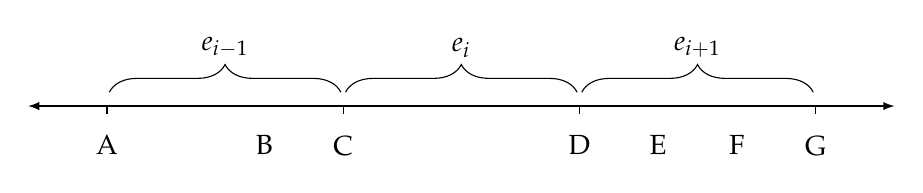
\begin{tikzpicture}
% axis
\draw[latex-latex] (0,0) -- (11,0) ;

% epoch braces
\draw [decorate,decoration={brace,amplitude=10pt} ,yshift=5pt] (1.03,0) -- (3.97,0)
  node [midway, above, yshift=9pt]{$e_{i-1}$};
\draw [decorate,decoration={brace,amplitude=10pt} ,yshift=5pt] (4.03,0) -- (6.97,0)
  node [midway, above, yshift=9pt]{$e_{i}$};
\draw [decorate,decoration={brace,amplitude=10pt} ,yshift=5pt] (7.03,0) -- (9.97,0)
  node [midway, above, yshift=9pt]{$e_{i+1}$};

% epoch boundaries
\foreach \x in  {1,4,7,10}
  \draw[shift={(\x,0)}] (0pt,0pt) -- (0pt,-3pt);

\node at (1,-0.5) {A};
\node at (3,-0.5) {B};
\node at (4,-0.5) {C};
\node at (7,-0.5) {D};
\node at (8,-0.5) {E};
\node at (9,-0.5) {F};
\node at (10,-0.5) {G};

\end{tikzpicture}

We must therefore store the last three stake distributions.
The mnemonic ``mark, set, go'' will be used to keep
track of the snapshots, where the label ``mark'' refers to the most recent snapshot,
and ``go'' refers to the snapshot that is ready to be used in the reward calculation.
In the above diagram, the snapshot taken at (A) is labeled ``mark'' during epoch $e_{i-1}$,
``set'' during epoch $e_i$ and ``go'' during epoch $e_{i+1}$. At (G) the snapshot
taken at (A) is no longer needed and will be discarded.

The two main transition systems in this section are:
\begin{itemize}
  \item The transition system named $\mathsf{EPOCH}$, which is defined in
    Section~\ref{sec:total-epoch}, covers what happens at the epoch boundary,
    such as at (A), (C), (D) and (G).
  \item The transition named $\mathsf{RUPD}$, which is defined in
    Section~\ref{sec:reward-update-trans}, covers the reward calculation that
    happens between (E) and (F).
\end{itemize}


\begin{note}
  Between time D and E we are concerned with chain growth and stability.
  Therefore this duration can be stated as 2k blocks (to state it in slots requires details about
  the particular version of the Ouroboros protocol). The duration between F and G is also 2k blocks.
  Between E and F a single honest block is enough to ensure a random nonce.
\end{note}

\subsection{Helper Functions and Accounting Fields}
\label{sec:stake-dist-helpers}

Figure~\ref{fig:funcs:epoch-helper-rewards} defines four helper functions needed
throughout the rest of the section.

\begin{itemize}
  \item The function $\fun{obligation}$ calculates the the minimal amount of coin needed to
    pay out all deposit refunds, as of the current slot.
  \item The function $\fun{poolRefunds}$ is used to calculate the total refunds
    that must be distributed for stake pools scheduled to retire.
    Note that this calculation takes a slot number corresponding to the epoch boundary slot
    when the calculation is performed.  The returned map maps pool operator hashkeys to the
    refunds, which will ultimately be returned to the registered reward account.
  \item The function $\fun{poolStake}$ filters the stake distribution to one stake pool.
\end{itemize}


%%
%% Figure - Helper Functions for Epoch Rules
%%
\begin{figure}[htb]
  \emph{Total possible refunds}
  \begin{align*}
    & \fun{obligation} \in \PParams \to \StakeCreds \to \StakePools \to \Slot \to \Coin \\
    & \obligation{pp}{stkCreds}{stpools}{cslot} =\\
    & \sum\limits_{(\_ \mapsto s) \in \var{stkCreds}}
      \refund{d_{\mathsf{val}}}{d_{\min}}{\lambda_d}{(\slotminus{cslot}{s})}
      + \sum\limits_{(\_ \mapsto s) \in \var{stpools}}
      \refund{p_{\mathsf{val}}}{p_{\min}}{\lambda_p}{(\slotminus{cslot}{s})} \\
    &
      \begin{array}{lr@{~=~}l}
        \where
          & \dval,~d_{\min},~\lambda_d
          & \fun{keyDeposit}~\var{pp},~\fun{keyMinRefund}~\var{pp},~\fun{keyDecayRate}~\var{pp}
          \\
          & p_{\mathsf{val}},~p_{\min},~\lambda_p
          & \fun{poolDeposit}~\var{pp},~\fun{poolMinRefund}~\var{pp},~\fun{poolDecayRate}~\var{pp}
      \end{array}\\
  \end{align*}
  \emph{Pool refunds}
  \begin{align*}
      & \fun{poolRefunds} \in \PParams \to (\KeyHash_{pool} \mapsto \Epoch) \to \Slot \to
      (\KeyHash_{pool} \mapsto \Coin) \\
      & \poolRefunds{pp}{retiring}{cslot} = \left\{
        \var{hk}\mapsto
          \refund{p_{\mathsf{val}}}{p_{\min}}{\lambda_p}{(\slotminus{cslot}{(\fun{slot}~e)})}
          \mid
          \var{hk}\mapsto e\in\var{retiring}
        \right\}\\
      & \where p_{\mathsf{val}},~p_{\min},~\lambda_p =
          \fun{poolDeposit}~\var{pp},~\fun{poolMinRefund}~\var{pp},~\fun{poolDecayRate}~\var{pp} \\
  \end{align*}

  \emph{Filter Stake to one Pool}
  \begin{align*}
      & \fun{poolStake} \in \KeyHash_{pool} \to (\KeyHash_{stake} \mapsto \KeyHash_{pool})
        \to \Stake \to \Stake \\
      & \poolStake{hk}{delegs}{stake} =
        \dom{(\var{delegs}\restrictrange\{hk\})\restrictdom\var{stake}}
  \end{align*}

  \caption{Helper Functions used in Rewards and Epoch Boundary}
  \label{fig:funcs:epoch-helper-rewards}
\end{figure}


The Figure~\ref{fig:defs:accounting} lists the accounting fields, denoted by $\Acnt$,
which will be used throughout this section. It consists of:
\begin{itemize}
  \item The value $\var{treasury}$ tracks the amount of coin currently stored in the treasury.
    Initially there will be no way to remove these funds.
  \item The value $\var{reserves}$ tracks the amount of coin currently stored in the reserves.
    This pot is used to pay rewards.
\end{itemize}
More will be said about the general accounting system in Section~\ref{sec:reward-calc}.

%%
%% Figure - Accounting fields
%%
\begin{figure}[htb]
  \emph{Accounting Fields}
  \begin{equation*}
    \Acnt =
    \left(
      \begin{array}{r@{~\in~}ll}
        \var{treasury} & \Coin & \text{treasury pot}\\
        \var{reserves} & \Coin & \text{reserve pot}\\
      \end{array}
    \right)
  \end{equation*}
  %
  \caption{Accounting fields}
  \label{fig:defs:accounting}
\end{figure}


\subsection{Stake Distribution Calculation}
\label{sec:stake-dist-calc}

This section defines the stake distribution calculations.
Figure~\ref{fig:epoch-defs} introduces three new derived types:
\begin{itemize}
  \item $\type{BlocksMade}$ represents the number of blocks each stake pool produced
    during an epoch.
  \item $\type{Stake}$ represents the amount of stake (in $\type{Coin}$) controlled by each
    stake pool.
\end{itemize}

%%
%% Figure - Epoch Abstract Types
%%
\begin{figure}[htb]
  \emph{Derived types}
  %
  \begin{equation*}
    \begin{array}{r@{~\in~}l@{\qquad=\qquad}lr}
      \var{blocks}
      & \BlocksMade
      & \KeyHash_{pool} \mapsto \N
      & \text{blocks made by stake pools} \\
      \var{stake}
      & \Stake
      & \Credential \mapsto \Coin
      & \text{stake} \\
    \end{array}
  \end{equation*}
  \caption{Epoch definitions}
  \label{fig:epoch-defs}
\end{figure}

The stake distribution calculation is given in Figure~\ref{fig:functions:stake-distribution}.

\begin{itemize}
\item $\fun{aggregate_{+}}$ takes a relation on $A\times B$, where $B$ is any
  monoid $(B,+,e)$ and returns a map from each $a\in A$ to the ``sum'' (using
  the monoidal $+$ operation) of all $b\in B$ such that $(a, b)\in A\times B$.
\item $\fun{stakeDistr}$ uses the $\fun{aggregate_{+}}$ function and several relations to
    compute the stake distribution, mapping each hashkey to the total coin under its control.
    Keys that are not both registered and delegated are filtered out.
    The relation passed to $\fun{aggregate_{+}}$ is made up of:
    \begin{itemize}
      \item $\fun{stakeCred_b}^{-1}$, relating credentials to (base) addresses
      \item $\left(\fun{addrPtr}\circ\var{ptr}\right)^{-1}$, relating credentials to (pointer)
        addresses
      \item $\range{utxo}$, relating addresses to coins
      \item $\fun{stakeCred_r}^{-1}\circ\var{rewards}$, relating (reward) addresses to coins
    \end{itemize}
    The notation for relations is explained in Section~\ref{sec:notation-shelley}.
\end{itemize}

%%
%% Figure Functions for Stake Distribution
%%
\begin{figure}[htb]
  \emph{Aggregation (for a monoid B)}
  %
  \begin{align*}
      & \fun{aggregate_{+}} \in \powerset{(A \times B)} \to (A\mapsto B) \\
      & \fun{aggregate_{+}}~\var{R} = \left\{a\mapsto \sum_{(a,b)\in\var{R}}b
          ~\mid~a\in\dom\var{R}\right\} \\
  \end{align*}
  %
  \emph{Stake Distribution (using functions and maps as relations)}
  %
  \begin{align*}
      & \fun{stakeDistr} \in \UTxO \to \DState \to \PState \to \Stake \\
      & \fun{stakeDistr}~{utxo}~{dstate}~{pstate} =
      (\dom{\var{activeDelegs}})\restrictdom\left(\fun{aggregate_{+}}~\var{stakeRelation}\right)\\
      & \where \\
      & ~~~~ (\var{stkCreds},~\var{rewards},~\var{delegations},~\var{ptrs},~\wcard,~\wcard)
        = \var{dstate} \\
      & ~~~~ (\var{stpools},~\wcard,~\wcard) = \var{pstate} \\
      & ~~~~ \var{stakeRelation} = \left(
        \left(\fun{stakeCred_b}^{-1}\cup\left(\fun{addrPtr}\circ\var{ptr}\right)^{-1}\right)
        \circ\left(\range{\var{utxo}}\right)
        \right)
        \cup \left(\fun{stakeCred_r}^{-1}\circ\var{rewards}\right) \\
      & ~~~~ \var{activeDelegs} =
               (\dom{stkCreds}) \restrictdom \var{delegations} \restrictrange (\dom{stpools}) \\
  \end{align*}

  \caption{Stake Distribution Function}
  \label{fig:functions:stake-distribution}
\end{figure}

\clearpage

\subsection{Snapshot Transition}
\label{sec:snapshots}

The state transition types for stake distribution snapshots are given in
Figure~\ref{fig:ts-types:snapshot}.
Each snapshot consists of:
\begin{itemize}
  \item $\var{stake}$, a stake distribution, which is defined in
    Figure~\ref{fig:epoch-defs} as a mapping of credentials to coin.
  \item $\var{delegations}$, a delegation map, mapping credentials to stake pools.
  \item $\var{poolParameters}$, storing the pool parameters of each stake pool.
\end{itemize}

The type $\type{\Snapshots}$ contains the
information needing to be saved on the epoch boundary:
\begin{itemize}
  \item $\var{pstake_{mark}}$, $\var{pstake_{set}}$ and $\var{pstake_{go}}$ are the three
    snapshots as explained in Section~\ref{sec:reward-overview}.
  \item $\var{feeSS}$ stores the fees and decayed deposit amounts at the epoch boundary.
\end{itemize}

%%
%% Figure - Snapshots Defs
%%
\begin{figure}[htb]
  \emph{Snapshot environment}
  \begin{equation*}
    \SnapshotEnv =
    \left(
      \begin{array}{r@{~\in~}ll}
        \var{pp} & \PParams & \text{protocol parameters}\\
        \var{dstate} & \DState & \text{delegation state}\\
        \var{pstate} & \PState & \text{pool state}\\
      \end{array}
    \right)
  \end{equation*}
  %
  \emph{Snapshots}
  \begin{equation*}
    \Snapshot =
    \left(
      \begin{array}{r@{~\in~}ll}
        \var{stake} & \Stake & \text{stake distribution}\\
        \var{delegations} & \Credential\mapsto\KeyHash_{pool}
                          & \text{stake delegations}\\
        \var{poolParameters} & \KeyHash_{pool} \mapsto \PoolParam & \text{pool parameters }\\
      \end{array}
    \right)
  \end{equation*}

  \begin{equation*}
    \Snapshots =
    \left(
      \begin{array}{r@{~\in~}ll}
        \var{pstake_{mark}} & \Snapshot & \text{newest stake}\\
        \var{pstake_{set}}  & \Snapshot & \text{middle stake}\\
        \var{pstake_{go}}   & \Snapshot & \text{oldest stake}\\
        \var{feeSS} & \Coin & \text{fee snapshot}\\
      \end{array}
    \right)
  \end{equation*}
  %
  \emph{Snapshot States}
  \begin{equation*}
    \SnapshotState =
    \left(
      \begin{array}{r@{~\in~}ll}
        \var{ss} & \Snapshots & \text{snapshots}\\
        \var{utxoSt} & \UTxOState & \text{utxo state}\\
      \end{array}
    \right)
  \end{equation*}
  %
  \emph{Snapshot transitions}
  \begin{equation*}
    \_ \vdash
    \var{\_} \trans{snap}{\_} \var{\_}
    \subseteq \powerset (\SnapshotEnv \times \SnapshotState \times \Epoch \times \SnapshotState)
  \end{equation*}
  %
  \caption{Snapshot transition-system types}
  \label{fig:ts-types:snapshot}
\end{figure}

The snapshot transition rule is given in Figure~\ref{fig:rules:snapshot}.
This transition has no preconditions and results in the following state change:

\begin{itemize}
  \item The oldest snapshot is replaced with the penultimate one.
  \item The penultimate snapshot is replaced with the newest one.
  \item The newest snapshot is replaced with one just calculated.
  \item The fees and decayed deposits are stored in $\var{feeSS}$. Note that this value will not
    change between epochs, unlike the $\var{fees}$ and $\var{deposits}$ values in the UTxO state.
  \item In the UTxO state, the decayed deposit amounts are moved from the deposit pot
    to the fee pool. Note that in the reward transition (Section~\ref{sec:reward-calc}),
    the value $\var{feeSS}$ will be removed from the fee pot in the UTxO state.
    The decay is calculated based on \textit{the first slot in the upcoming epoch}.
\end{itemize}

%%
%% Figure - Snapshot Rule
%%
\begin{figure}[htb]
  \begin{equation}\label{eq:snapshot}
    \inference[Snapshot]
    {
      {
      \begin{array}{r@{~\leteq~}l}
        (\var{stkCreds},~\wcard,~\var{delegations},~\wcard,~\wcard,~\wcard) & \var{dstate}\\
        (\var{stpools},~\var{poolParams},~\wcard) & \var{pstate}\\
        \var{stake} & \stakeDistr{utxo}{dstate}{pstate} \\
        \var{slot} & \firstSlot{e} \\
        \var{oblg} & \obligation{pp}{stkCreds}{stpools}{slot} \\
        \var{decayed} & \var{deposits} - \var{oblg} \\
      \end{array}
      }
    }
    {
      \begin{array}{r}
        \var{pp} \\
        \var{dstate} \\
        \var{pstate} \\
      \end{array}
      \vdash
      \left(
        \begin{array}{r}
          \var{pstake_{mark}}\\
          \var{pstake_{set}}\\
          \var{pstake_{go}}\\
          \var{feeSS} \\
          ~ \\
          \var{utxo} \\
          \var{deposits} \\
          \var{fees} \\
          \var{pup} \\
        \end{array}
      \right)
      \trans{snap}{e}
      \left(
        \begin{array}{r}
          \varUpdate{(\var{stake},~\var{delegations},~\var{poolParams})} \\
          \varUpdate{\var{pstake_{mark}}} \\
          \varUpdate{\var{pstake_{set}}} \\
          \varUpdate{\var{fees} + \var{decayed}} \\
          ~ \\
          \var{utxo} \\
          \varUpdate{\var{oblg}} \\
          \varUpdate{\var{fees} + \var{decayed}} \\
          \var{pup} \\
        \end{array}
      \right)
    }
  \end{equation}
  \caption{Snapshot Inference Rule}
  \label{fig:rules:snapshot}
\end{figure}

\clearpage

\subsection{Pool Reaping Transition}
\label{sec:pool-reap}

Figure~\ref{fig:ts-types:pool-reap} defines the types for the pool reap transition,
which is responsible for removing pools slated for retirement in the given epoch.

%%
%% Figure - Pool Reap Defs
%%
\begin{figure}[htb]
  \emph{Pool Reap State}
  \begin{equation*}
    \PlReapState =
    \left(
      \begin{array}{r@{~\in~}ll}
        \var{utxoSt} & \UTxOState & \text{utxo state}\\
        \var{acnt} & \Acnt & \text{accounting}\\
        \var{dstate} & \DState & \text{delegation state}\\
        \var{pstate} & \PState & \text{pool state}\\
      \end{array}
    \right)
  \end{equation*}
  %
  \emph{Pool Reap transitions}
  \begin{equation*}
    \_ \vdash \_ \trans{poolreap}{\_} \_ \in
    \powerset (\PParams \times \PlReapState \times \Epoch \times \PlReapState)
  \end{equation*}
  %
  \caption{Pool Reap Transition}
  \label{fig:ts-types:pool-reap}
\end{figure}


The pool-reap transition rule is given in Figure~\ref{fig:rules:pool-reap}.
This transition has no preconditions and results in the following state change:

\begin{itemize}
  \item For each retiring pool, the refund for the pool registration deposit is added to the
    pool's registered reward account, provided the reward account is still registered.
  \item The sum of all the refunds attached to unregistered reward accounts are added to the
    treasury.
  \item The deposit pool is reduced by the amount of claimed and unclaimed refunds.
  \item Any delegation to a retiring pool is removed.
  \item Each retiring pool is removed from all four maps in the pool state.
\end{itemize}

%%
%% Figure - Pool Reap Rule
%%
\begin{figure}[htb]
  \begin{equation}\label{eq:pool-reap}
    \inference[Pool-Reap]
    {
      {
      \begin{array}{r@{~\leteq~}l}
        \var{retired} & \dom{(\var{retiring}^{-1}~\var{e})} \\
        \var{pr} & \poolRefunds{pp}{(\var{retired}\restrictdom\var{stpools})}{(\firstSlot{e})} \\
        \var{rewardAcnts}
                 & \{\var{hk}\mapsto \fun{poolRAcnt}~\var{pool} \mid
                   \var{hk}\mapsto\var{pool} \in \var{retired}\restrictdom\var{poolParams} \} \\
        \var{rewardAcnts'} & \left\{
                        a \mapsto c
                        \mathrel{\Bigg|}
                        \begin{array}{r@{~\in~}l}
                          \var{hk} \mapsto c & \var{pr}, \\
                          \var{hk}\mapsto\var{a} & \var{rewardAcnts} \\
                        \end{array}
                      \right\} \\
        \var{refunds} & \dom{rewards}\restrictdom\var{rewardAcnts'} \\
        \var{mRefunds} & \dom{rewards}\subtractdom\var{rewardAcnts'} \\
        \var{refunded} & \sum\limits_{\wcard\mapsto c\in\var{refunds}} c \\
        \var{unclaimed} & \sum\limits_{\wcard\mapsto c\in\var{mRefunds}} c \\
      \end{array}
      }
    }
    {
      \var{pp}
      \vdash
      \left(
        \begin{array}{r}
          \var{utxo} \\
          \var{deposits} \\
          \var{fees} \\
          \var{ups} \\
          ~ \\
          \var{treasury} \\
          \var{reserves} \\
          ~ \\
          \var{stkCreds} \\
          \var{rewards} \\
          \var{delegations} \\
          \var{ptrs} \\
          \var{genDelegs} \\
          \var{i_{rwd}} \\
          ~ \\
          \var{stpools} \\
          \var{poolParams} \\
          \var{retiring} \\
        \end{array}
      \right)
      \trans{poolreap}{e}
      \left(
        \begin{array}{rcl}
          \var{utxo} \\
          \varUpdate{\var{deposits}}
          & \varUpdate{-}
          & \varUpdate{(\var{unclaimed} + \var{refunded})} \\
          \var{fees} \\
          \var{ups} \\
          ~ \\
          \varUpdate{\var{treasury}} & \varUpdate{+} & \varUpdate{\var{unclaimed}} \\
          \var{reserves} \\
          ~ \\
          \var{stkCreds} \\
          \varUpdate{\var{rewards}} & \varUpdate{\unionoverridePlus} & \varUpdate{\var{refunds}} \\
          \varUpdate{\var{delegations}} & \varUpdate{\subtractrange} & \varUpdate{\var{retired}} \\
          \var{ptrs} \\
          \var{genDelegs} \\
          \var{i_{rwd}}\\
          ~ \\
          \varUpdate{\var{retired}} & \varUpdate{\subtractdom} & \varUpdate{\var{stpools}} \\
          \varUpdate{\var{retired}} & \varUpdate{\subtractdom} & \varUpdate{\var{poolParams}} \\
          \varUpdate{\var{retired}} & \varUpdate{\subtractdom} & \varUpdate{\var{retiring}} \\
        \end{array}
      \right)
    }
  \end{equation}
  \caption{Pool Reap Inference Rule}
  \label{fig:rules:pool-reap}
\end{figure}

\clearpage

\subsection{Protocol Parameters Update Transition}
\label{sec:pparam-update}

Finally, reaching the epoch boundary may trigger a change in the protocol
parameters. The protocol parameters environment consists of the new
protocol parameters and the delegation and pool states.
The state change is a change of the $\UTxOState$, the $\Acnt$ states and the current $\PParams$.
The type of this state transition is given in Figure~\ref{fig:ts-types:new-proto-param}.

%%
%% Figure - New Proto Param Defs
%%
\begin{figure}[htb]
  \emph{New Proto Param environment}
  \begin{equation*}
    \NewPParamEnv =
    \left(
      \begin{array}{r@{~\in~}ll}
        \var{pp_{new}} & \PParams^? & \text{new protocol parameters}\\
        \var{dstate} & \DState & \text{delegation state}\\
        \var{pstate} & \PState & \text{pool state}\\
      \end{array}
    \right)
  \end{equation*}
  %
  \emph{New Proto Param States}
  \begin{equation*}
    \NewPParamState =
    \left(
      \begin{array}{r@{~\in~}ll}
        \var{utxoSt} & \UTxOState & \text{utxo state}\\
        \var{acnt} & \Acnt & \text{accounting}\\
        \var{pp} & \PParams & \text{current protocol parameters}\\
      \end{array}
    \right)
  \end{equation*}
  %
  \emph{New Proto Param transitions}
  \begin{equation*}
    \_ \vdash
    \var{\_} \trans{newpp}{\_} \var{\_}
    \subseteq \powerset (\NewPParamEnv \times \NewPParamState \times \Epoch \times \NewPParamState)
  \end{equation*}
  %
  \caption{New Proto Param transition-system types}
  \label{fig:ts-types:new-proto-param}
\end{figure}


Figure~\ref{fig:rules:new-proto-param} defines the new protocol parameter transition.
The transition has two rules, depending on whether or not the new protocol parameters
meet some requirements.
In particular, we require that the new parameters would not incur a debt of the system that
can not be covered by the reserves, and that the max block size is greater than the sum of the
max transaction size and the max header size.
If the requirements are met, the new protocol parameters are accepted, the proposal is reset,
and the reserves are adjusted to account for changes in the deposits.
Otherwise, the only change is that the proposal is reset.

Regarding adjusting the reserves for changes in the deposits, one of three things happens:

\begin{itemize}
  \item If the new protocol parameters mean that \textbf{fewer} funds are required in the
    deposit pot to cover all possible refunds, then the excess is moved to the reserves.

  \item If the new protocol parameters mean that \textbf{more} funds are required in the
    deposit pot to cover all possible refunds and the difference is \textbf{less} than
    the reserve pot, then funds are moved from the reserve pot to cover the difference.

  \item If the new protocol parameters mean that \textbf{more} funds are required in the
    deposit pot to cover all possible refunds and the difference is \textbf{more} than
    the reserve pot, then Rule~\ref{eq:new-pc-denied} meets the precondition and the
    only change of state is that the update proposals are reset.
\end{itemize}

Note that here, unlike most of the inference rules in this document,
the $\var{utxoSt'}$ and the $\var{acnt'}$ do not come from valid UTxO or
accounts transitions in the antecedent. We simply define the consequent
transition using these directly (instead of listing all the fields in both
states in the consequent transition). It is done this way here
for ease of reading.

%%
%% Figure - New Proto Param Rule
%%
\begin{figure}[htb]
  \begin{equation}\label{eq:new-pc-accepted}
    \hspace{-0.3cm}
    \inference[New-Proto-Param-Accept]
    {
      \var{pp_{new}}\neq\Nothing \\~\\
      {\begin{array}{rcl}
         \var{slot} & \leteq & \firstSlot{e} \\
         \var{oblg_{cur}} & \leteq & \obligation{pp}{stkCreds}{stpools}{slot} \\
         \var{oblg_{new}} & \leteq & \obligation{pp_{new}}{stkCreds}{stpools}{slot} \\
         \var{(\wcard,~\wcard,~\wcard,~\wcard,~\wcard,~\wcard,~\var{i_{rwd}})} &
                                                                                      \leteq
                              & \var{dstate}\\
         \var{diff} & \leteq & \var{oblg_{cur}} - \var{oblg_{new}}\\
         (\var{utxo},~\var{deposits},~\var{fees},~\var{ups}) & \leteq & \var{utxoSt} \\
         (\var{pup},~\var{aup},~\var{favs},~\var{avs}) & \leteq & \var{ups} \\
      \end{array}}
      \\~\\~\\
      \var{oblg_{cur}} = \var{deposits} \\
      \var{reserves} + \var{diff} \geq \sum\limits_{\wcard\mapsto\var{val}\in\var{i_{rwd}}} val \\
      \fun{maxTxSize}~\var{pp_{new}} + \fun{maxHeaderSize}~\var{pp_{new}} <
        \fun{maxBlockSize}~\var{pp_{new}}
      \\~\\
        \var{utxoSt'} \leteq
        \left(\var{utxo},~\varUpdate{oblg_{new}},~\var{fees}
        \left(\varUpdate{\emptyset},~\var{aup},~\var{favs},~\var{avs}\right)\right)
      \\~\\
      (\var{treasury},~\var{reserves})\leteq \var{acnt} \\
      \var{acnt'} \leteq (\var{treasury},~\varUpdate{reserves + diff}) \\
    }
    {
      \begin{array}{l}
        \var{pp_{new}}\\
        \var{dstate}\\
        \var{pstate}\\
      \end{array}
      \vdash
      \left(
        \begin{array}{r}
          \var{utxoSt} \\
          \var{acnt} \\
          \var{pp}
        \end{array}
      \right)
      \trans{newpp}{e}
      \left(
        \begin{array}{rcl}
          \varUpdate{utxoSt'}\\
          \varUpdate{acnt'} \\
          \varUpdate{\var{pp_{new}}} \\
        \end{array}
      \right)
    }
  \end{equation}

  \nextdef

  \begin{equation}\label{eq:new-pc-denied}
    \inference[New-Proto-Param-Denied]
    {
      \left({\begin{array}{c}
            \var{pp_{new}}=\Nothing \\
        \lor \\
        \var{reserves} + \var{diff} < \sum\limits_{\wcard\mapsto\var{val}\in\var{i_{rwd}}} val\\
        \lor \\
        \fun{maxTxSize}~\var{pp_{new}} + \fun{maxHeaderSize}~\var{pp_{new}} \geq
          \fun{maxBlockSize}~\var{pp_{new}}
      \end{array}}\right)
      \\~\\~\\
      {\begin{array}{rcl}
          \var{slot} & \leteq & \firstSlot{e} \\
          \var{oblg_{cur}} & \leteq & \obligation{pp}{stkCreds}{stpools}{slot} \\
          \var{oblg_{new}} & \leteq & \obligation{pp_{new}}{stkCreds}{stpools}{slot} \\
         \var{(\wcard,~\wcard,~\wcard,~\wcard,~\wcard,~\wcard,~\var{i_{rwd}})} &
                                                                                 \leteq
                              & \var{dstate}\\
         \var{diff} & \leteq & \var{oblg_{cur}} - \var{oblg_{new}}
      \end{array}}
      \\~\\~\\
      \left(\var{utxo},~\var{oblg},~\var{fees}
        \left(\var{pup},~\var{aup},~\var{favs},~\var{avs}\right)\right)
        \leteq \var{utxoSt} \\
        \var{utxoSt'} \leteq
        \left(\var{utxo},~\var{oblg},~\var{fees}
        \left(\varUpdate{\emptyset},~\var{aup},~\var{favs},~\var{avs}\right)\right)
    }
    {
      \begin{array}{l}
        \var{pp_{new}}\\
        \var{dstate}\\
        \var{pstate}\\
      \end{array}
      \vdash
      \left(
        \begin{array}{r}
          \var{utxoSt} \\
          \var{acnt} \\
          \var{pp}
        \end{array}
      \right)
      \trans{newpp}{e}
      \left(
        \begin{array}{rcl}
          \varUpdate{utxoSt'}\\
          \var{acnt} \\
          \var{pp}
        \end{array}
      \right)
    }
  \end{equation}
  \caption{New Proto Param Inference Rule}
  \label{fig:rules:new-proto-param}
\end{figure}

\clearpage

\subsection{Complete Epoch Boundary Transition}
\label{sec:total-epoch}

Finally, it is possible to define the complete epoch boundary transition type,
which is defined in Figure~\ref{fig:ts-types:epoch}.
The transition has no evironment.
The state is made up of the the accounting state, the snapshots, the ledger state and the
protocol parameters.
The transition uses a helper function $\fun{votedValue}$ which returns
the consensus value of update proposals in the event that consensus is met.
\textbf{Note that} $\fun{votedValue}$
\textbf{is only well-defined if } $\Quorum$
\textbf{is greater than half the number of core nodes, i.e.}
$\Quorum > |\var{genDelegs}|/2$ \textbf{.}

%%
%% Figure - Epoch Defs
%%
\begin{figure}[htb]
  \emph{Epoch States}
  \begin{equation*}
    \EpochState =
    \left(
      \begin{array}{r@{~\in~}ll}
        \var{acnt} & \Acnt & \text{accounting}\\
        \var{ss} & \Snapshots & \text{snapshots}\\
        \var{ls} & \LState & \text{ledger state}\\
        \var{prevPp} & \PParams & \text{previous protocol parameters}\\
        \var{pp} & \PParams & \text{protocol parameters}\\
      \end{array}
    \right)
  \end{equation*}
  %
  \emph{Epoch transitions}
  \begin{equation*}
    \vdash
    \var{\_} \trans{epoch}{\_} \var{\_}
    \subseteq \powerset (\EpochState \times \Epoch \times \EpochState)
  \end{equation*}
  %
  \emph{Accessor Functions}
  \begin{equation*}
    \begin{array}{r@{~\in~}lr}
      \fun{getIR} & \EpochState \to (\StakeCredential \mapsto \Coin)
                  & \text{get instantaneous rewards} \\
    \end{array}
  \end{equation*}
  %
  \emph{Helper Functions}
  \begin{align*}
      & \fun{votedValue} \in (\KeyHashGen\mapsto\PParamsUpdate) \to \PParamsUpdate^?\\
      & \fun{votedValue}~\var{vs} =
        \begin{cases}
          p & \exists p\in\range{vs}~(|vs\restrictrange p|\geq \Quorum) \\
          \Nothing & \text{otherwise} \\
        \end{cases}
  \end{align*}
  %
  \caption{Epoch transition-system types}
  \label{fig:ts-types:epoch}
\end{figure}


The epoch transition rule calls $\mathsf{SNAP}$, $\mathsf{POOLREAP}$ and $\mathsf{NEWPP}$
in sequence. It also stores the previous protocol parameters in $\var{prevPp}$.
The previous protocol parameters will be used for the reward calculation in the upcoming epoch,
note that they correspond to the epoch for which the rewards are being calculated.
Additionally, this transition also adopts the pool parameters $\var{fPoolParams}$
corresponding to the pool re-registration certificates which we submitted late in the ending epoch.
The ordering of these rules is important.
The stake pools which will be updated by $\var{fPoolParams}$ or
reaped during the $\mathsf{POOLREAP}$ transition must still be a
part of the new snapshot, and so $\mathsf{SNAP}$ must occur before these two actions.
Moreover, $\mathsf{SNAP}$ sets the deposit pot equal to current obligation,
which is a property that is preserved by $\mathsf{POOLREAP}$ and which
is necessary for the preservation of Ada property in the $ \mathsf{NEWPP}$ transition.

%%
%% Figure - Epoch Rule
%%
\begin{figure}[htb]
  \begin{equation}\label{eq:epoch}
    \inference[Epoch]
    {
      (\var{utxoSt},~(\var{dstate},~\var{pstate}))\leteq\var{ls} \\
      {
        \begin{array}{r}
          \var{pp}\\
          \var{dstate} \\
          \var{pstate} \\
        \end{array}
      }
      \vdash
      {
        \left(
          {
            \begin{array}{r}
              \var{ss} \\
              \var{utxoSt} \\
            \end{array}
          }
        \right)
      }
      \trans{\hyperref[fig:rules:snapshot]{snap}}{e}
      {
        \left(
          {
            \begin{array}{r}
              \var{ss'} \\
              \var{utxoSt'} \\
            \end{array}
          }
        \right)
      }
      \\~\\~\\
      (\var{stpools},~\var{poolParams},~\var{fPoolParams},~\var{retiring})\leteq\var{pstate}
      \\
      \var{pstate'}\leteq(\var{stpools},~\var{poolParams}\unionoverrideRight\var{fPoolParams},
      ~\emptyset,~\var{retiring})
      \\~\\~\\
      \var{pp}
      \vdash
      \left(
        {
          \begin{array}{r}
            \var{utxoSt'} \\
            \var{acnt} \\
            \var{dstate} \\
            \var{pstate'} \\
          \end{array}
        }
      \right)
      \trans{\hyperref[fig:rules:pool-reap]{poolreap}}{e}
      \left(
      {
        \begin{array}{rcl}
            \var{utxoSt''} \\
            \var{acnt'} \\
            \var{dstate'} \\
            \var{pstate''} \\
        \end{array}
      }
      \right)
      \\~\\~\\
      \var{(\wcard,~\wcard,~\wcard,~\var{pup})}\leteq\var{utxoSt'}\\
      \var{pp_{new}}\leteq\var{pp}\unionoverrideRight
      \fun{votedValue}~\var{pup}\\
      {
        \begin{array}{r}
          \var{pp_{new}}\\
          \var{dstate'}\\
          \var{pstate''}\\
        \end{array}
      }
      \vdash
      \left(
        {
          \begin{array}{r}
            \var{utxoSt''} \\
            \var{acnt'} \\
            \var{pp}\\
          \end{array}
        }
      \right)
      \trans{\hyperref[fig:rules:new-proto-param]{newpp}}{e}
      \left(
      {
        \begin{array}{rcl}
            \var{utxoSt'''} \\
            \var{acnt''} \\
            \var{pp'}\\
        \end{array}
      }
      \right)
      \\~\\~\\
      \var{ls}' \leteq (\var{utxoSt}''',~(\var{dstate}',~\var{pstate}''))
    }
    {
      \vdash
      \left(
      \begin{array}{r}
        \var{acnt} \\
        \var{ss} \\
        \var{ls} \\
        \var{prevPp} \\
        \var{pp} \\
      \end{array}
      \right)
      \trans{epoch}{e}
      \left(
      \begin{array}{rcl}
        \varUpdate{\var{acnt''}} \\
        \varUpdate{\var{ss'}} \\
        \varUpdate{\var{ls'}} \\
        \varUpdate{\var{pp}} \\
        \varUpdate{\var{pp'}} \\
      \end{array}
      \right)
    }
  \end{equation}
  \caption{Epoch Inference Rule}
  \label{fig:rules:epoch}
\end{figure}

\clearpage

\subsection{Rewards Distribution Calculation}
\label{sec:reward-dist}

This section defines the reward calculation for the proof of stake leader election.
Figure~\ref{fig:functions:rewards} defines the pool reward as described in section
5.5.2 of~\cite{delegation_design}.

\begin{itemize}
  \item The function $\fun{maxPool}$ gives the maximum reward a stake pool can receive in an epoch.
    This is a fraction of the total available rewards for the epoch.
    The result depends on the pool's relative stake, the pool's pledge and the following
    protocol parameters:
    \begin{itemize}
      \item $\var{a_0}$, the leader-stake influence
      \item $n_{opt}$, the optimal number of saturated stake pools
    \end{itemize}
  \item The function $\fun{poolReward}$ gives the total rewards available to be
    distributed to the members of the given pool. It depends on the protocol parameter $d$,
    the relative stake $\sigma$, the number $n$ of blocks the pool added to the chain and the
    total number $\overline{N}$ of blocks added to the chain in the last epoch.

\end{itemize}

%%
%% Figure - Functions for the Reward Calculation
%%
\begin{figure}[htb]
  \emph{Maximal Reward Function, called $f(s,\sigma)$ in section 5.5.2 of~\cite{delegation_design}}
  %
  \begin{align*}
      & \fun{maxPool} \in \PParams \to \Coin \to \unitInterval \to \unitInterval \to \Coin \\
      & \fun{maxPool}~\var{pp}~\var{R}~\sigma~\var{p_r} =
          ~~~\floor*{
             \frac{R}{1 + a_0}
             \cdot
             \left(
               \sigma' + p'\cdot a_0\cdot\frac{\sigma' - p'\frac{z_0-\sigma'}{z_0}}{z_0}
             \right)} \\
      & ~~~\where \\
      & ~~~~~~~a_0 = \fun{influence}~pp \\
      & ~~~~~~~n_{opt} = \fun{nopt}~pp \\
      & ~~~~~~~z_0 = 1/n_{opt} \\
      & ~~~~~~~\sigma'=\min(\sigma,~z_0) \\
      & ~~~~~~~p'=\min(p_r,~z_0) \\
  \end{align*}

  \emph{Actual Reward Function, called $\hat{f}$ in section 5.5.2 of~\cite{delegation_design}}
  %
  \begin{align*}
      & \fun{poolReward} \in \unitInterval \to \unitInterval \to \N \to \N \to \Coin \to \Coin \\
      & \poolReward{d}{\sigma}{n}{\overline{N}}{f} =
      \floor*{\overline{p}\cdot\var{f}}\\
      & ~~~\where \\
      & ~~~~~~~\overline{p} =
        \begin{cases}
          \frac{\beta}{\sigma} & \text{if } d < 0.8 \\
          1 & \text{otherwise}
        \end{cases} \\
      & ~~~~~~~\beta = \frac{n}{\max(1, \overline{N})} \\
  \end{align*}
  \caption{Functions used in the Reward Calculation}
  \label{fig:functions:rewards}
\end{figure}

\clearpage

Figure~\ref{fig:functions:reward-splitting} gives the calculation for
splitting the pool rewards with its members, as described in 6.5.2 of \cite{delegation_design}.
The portion of rewards allocated to the pool operator and owners is different
than that of the members.

\begin{itemize}
  \item The $\fun{r_{operator}}$ function calculates the leader reward, based on the pool cost,
    margin and the proportion of the pool's total stake.  Note that this reward will go to the
    reward account specified in the pool registration certificate.
  \item The $\fun{r_{member}}$ function calculates the member reward, proportionally to their
    stake after the cost and margin are removed.
\end{itemize}

%%
%% Figure - Functions for the Reward Splitting
%%
\begin{figure}[htb]
  \emph{Pool leader reward, from section 5.5.3 of \cite{delegation_design}}
  %
  \begin{align*}
      & \fun{r_{operator}} \in \Coin \to \PoolParam \to \unitInterval \to \unitIntervalNonNull \to \Coin \\
      & \lReward{\hat{f}}{pool}{s}{\sigma} =
        \begin{cases}
        \hat{f} & \hat{f} \leq c\\
        c + \floor*{(\hat{f} - c)\cdot\left(m + (1-m)\cdot\frac{s}{\sigma}\right) }&
        \text{otherwise.}
      \end{cases} \\
      & ~~~\where \\
      & ~~~~~~~c = \fun{poolCost}~pool \\
      & ~~~~~~~m = \fun{poolMargin}~pool \\
  \end{align*}

  \emph{Pool member reward, from section 5.5.3 of \cite{delegation_design}}
  %
  \begin{align*}
    & \fun{r_{member}} \in \Coin \to \PoolParam \to \unitInterval \to \unitIntervalNonNull \to \Coin \\
    & \mReward{\hat{f}}{pool}{t}{\sigma} =
      \begin{cases}
        0 & \hat{f} \leq c\\
        \floor*{(\hat{f} - c)\cdot(1-m)\cdot\frac{t}{\sigma}} &
        \text{otherwise.}
      \end{cases} \\
    & ~~~\where \\
    & ~~~~~~~c = \fun{poolCost}~pool \\
    & ~~~~~~~m = \fun{poolMargin}~pool \\
  \end{align*}

  \caption{Functions used in the Reward Splitting}
  \label{fig:functions:reward-splitting}
\end{figure}


Finally, the full reward calculation is presented in Figure~\ref{fig:functions:reward-calc}.
The calculation is done pool-by-pool.
\begin{itemize}
\item The $\fun{rewardOnePool}$ function calculates the rewards given out to
  each member of a given pool. The pool leader is identified by the stake
  credential of the pool operator. The function returns the rewards, calculated
  as follows:
    \begin{itemize}
      \item $\var{pstake}$, the total amount of stake controlled by the stake pool.
      \item $\var{ostake}$, the total amount of stake controlled by the stake pool operator
        and owners
      \item $\sigma$, the total proportion of stake controlled by the stake pool.
      \item $\overline{N}$, the expected number of blocks the pool should have produced.
      \item $\var{pledge}$, the pool's pledge in lovelace.
      \item $p_r$, the pool's pledge, as a proportion of active stake.
      \item $\var{maxP}$, maximum rewards the pool can claim if the pledge is met,
        and zero otherwise.
      \item $\var{poolR}$, the pool's actual reward, based on its performance.
      \item $\var{mRewards}$, the member's rewards as a mapping of reward accounts to coin.
      \item $\var{lReward}$, the leader's reward as coin.
      \item $\var{potentialRewards}$, the combination of $\var{mRewards}$ and $\var{lRewards}$.
      \item $\var{rewards}$, the restriction of $\var{potentialRewards}$ to the active
        reward accounts.
    \end{itemize}
  \item The $\fun{reward}$ function applies $\fun{rewardOnePool}$ to each registered stake pool.
\end{itemize}

%%
%% Figure - The Reward Calculation
%%
\begin{figure}[htb]
  \emph{Calculation to reward a single stake pool}
  %
  \begin{align*}
    & \fun{rewardOnePool} \in \PParams \to \Coin \to \N \to \N \to \KeyHash \to \PoolParam\\
      & ~~~\to \Stake \to \Coin \to \powerset{\AddrRWD}
           \to (\AddrRWD \mapsto \Coin) \\
      & \rewardOnePool{pp}{R}{n}{\overline{N}}{poolHK}{pool}{stake}{tot}{addrs_{rew}} =
          \var{rewards}\\
      & ~~~\where \\
      & ~~~~~~~\var{pstake} = \sum_{\_\mapsto c\in\var{stake}} c \\
      & ~~~~~~~\var{ostake} = \sum_{\substack{
        hk_\mapsto c\in\var{stake}\\
        hk\in(\fun{poolOwners}~\var{pool})\\
        }} c \\
      & ~~~~~~~\sigma = \var{pstake} / tot \\
      & ~~~~~~~\var{pledge} = \fun{poolPledge}~pool \\
      & ~~~~~~~p_{r} = \var{pledge} / \var{tot} \\
      & ~~~~~~~maxP =
      \begin{cases}
        \fun{maxPool}~\var{pp}~\var{R}~\sigma~\var{p_r}&
        \var{pledge} \leq \var{ostake}\\
        0 & \text{otherwise.}
      \end{cases} \\
      & ~~~~~~~\var{poolR} = \poolReward{(\fun{d}~pp)}{\sigma}{n}{\overline{N}}{maxP} \\
      & ~~~~~~~\var{mRewards} = \left\{
                                  \addrRw~hk\mapsto\mReward{poolR}{pool}{\frac{c}{tot}}{\sigma}
                                  ~\Big\vert~
                                  hk\mapsto c\in\var{stake},~~hk \neq\var{poolHK}
                               \right\}\\
      & ~~~~~~~\var{lReward} = \lReward{poolR}{pool}{\frac{\var{ostake}}{tot}}{\sigma} \\
      & ~~~~~~~\var{potentialRewards} =
                 \var{mRewards} \cup
                 \{(\fun{poolRAcnt}~\var{pool})\mapsto\var{lReward}\} \\
      & ~~~~~~~\var{rewards} = \var{addrs_{rew}}\restrictdom{\var{potentialRewards}} \\
  \end{align*}

  \emph{Calculation to reward all stake pools}
  %
  \begin{align*}
      & \fun{reward} \in \PParams \to \BlocksMade \to \Coin\to \powerset{\AddrRWD}
      \to (\KeyHash \mapsto \PoolParam) \\
      & ~~~\to \Stake \to (\KeyHash_{stake} \mapsto \KeyHash_{pool}) \to
      \Coin \to (\AddrRWD \mapsto \Coin)\\
      & \reward{pp}{blocks}{R}{addrs_{rew}}{poolParams}{stake}{delegs}{total}
          = \var{rewards}\\
      & ~~~\where \\
      & ~~~~~~~tot = \sum_{\_\mapsto c\in \var{stake}}c \\
      & ~~~~~~~\var{\overline{N}} = \sum_{\_\mapsto m\in blocks}m \\
      & ~~~~~~~pdata = \left\{
        hk\mapsto \left(p,~n,~\poolStake{hk}{delegs}{stake}\right)
        \mathrel{\Bigg|}
        \begin{array}{r@{\mapsto}c@{~\in~}l}
          hk & \var{p} & \var{poolParams} \\
          hk & \var{n} & \var{blocks} \\
        \end{array}
      \right\} \\
      & ~~~~~~~\var{results} = \left\{
        hk \mapsto \rewardOnePool{pp}{R}{n}{\overline{N}}{hk}{p}{s}{tot}{addrs_{rew}}
                 \mid
        hk\mapsto(p, n, s)\in\var{pdata} \right\} \\
      & ~~~~~~~\var{rewards} = \bigcup_{\wcard\mapsto\var{r}\in\var{results}}\var{r}
  \end{align*}
  \caption{The Reward Calculation}
  \label{fig:functions:reward-calc}
\end{figure}

\clearpage

\subsection{Reward Update Calculation}
\label{sec:reward-calc}

This section defines the calculation of a reward update.
A reward update is the information needed to account for the movement of lovelace
in the system due to paying out rewards.

Figure~\ref{fig:fund-preservation} captures the potential movement of funds in the entire system,
taking every transition system in this document into account.  Value is moved between
accounting pots, but the total amount of value in the system remains constant.
In particular, the red subgraph represents the inputs and outputs to
the ``reward pot'', a temporary variable used during the reward update calculation in
Figure~\ref{fig:functions:reward-update-creation}.
The blue arrows represent the movement of funds that pass through the ``reward pot''.


\begin{figure}[htb]
  \begin{center}
    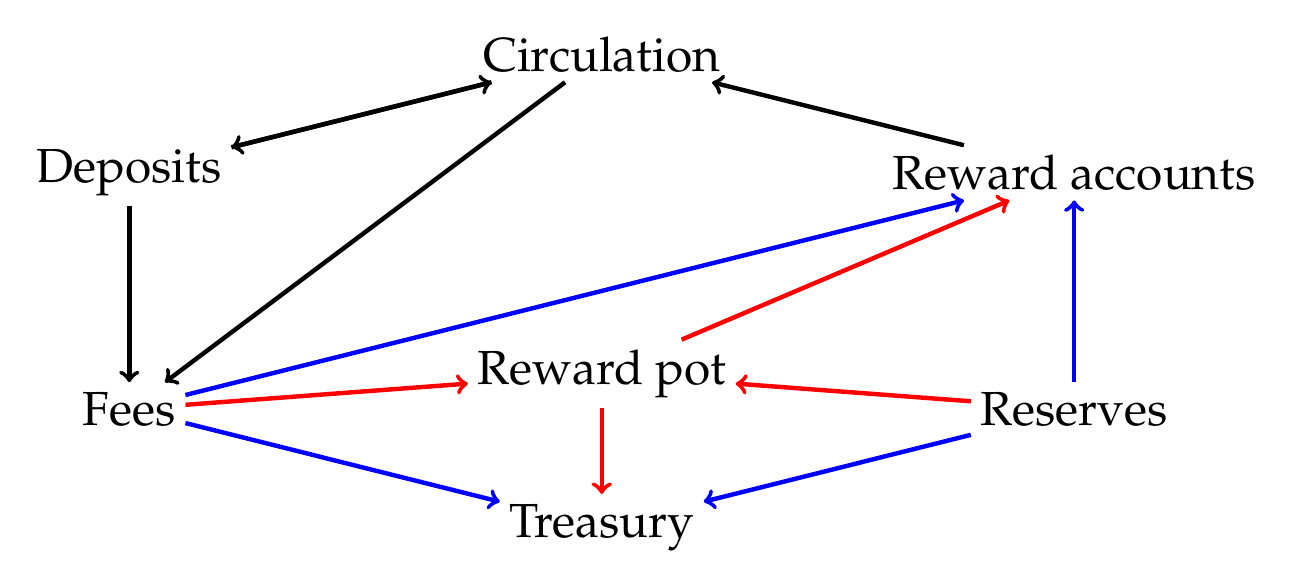
\begin{tikzpicture}
      [ x=30mm, y=30mm
      , direct/.style={black, draw}
      , implied/.style={blue, draw}
      , toTotPot/.style={red, draw}
      ]
    \node (C) at (3,2.5) {\LARGE Circulation};
    \node (R) at (5, 1) {\LARGE Reserves};
    \node (D) at (1, 2) {\LARGE Deposits};
    \node (FR) at (1,1) {\LARGE Fees};
    \node (RA) at (5, 2) {\LARGE Reward accounts};
    \node (T) at (3,0.5) {\LARGE Treasury};

    \draw[->, direct, ultra thick]
    (C) edge (D)
    (C) edge (FR)

    (D) edge (C)
    (D) edge (FR)

    (RA) edge (C);

    \draw[->, implied, ultra thick]
    (FR) edge (T)
    (FR) edge (RA)

    (R) edge (T)
    (R) edge (RA);

    \node (TP) at (3, 1.15) {\LARGE Reward pot};

    \draw[->, toTotPot, ultra thick]
    (FR) edge (TP)
    (R) edge (TP)

    (TP) edge (RA)
    (TP) edge (T);
    \end{tikzpicture}
  \end{center}
  \caption{Preservation of Value}
  \label{fig:fund-preservation}
\end{figure}

Figure~\ref{fig:defs:reward-update} defines a reward update.
It consists of four pots:
\begin{itemize}
  \item The change to the treasury. This will be a positive value.
  \item The change to the reserves. This will be a negative value.
  \item The map of new individual rewards (to be added to the existing rewards).
  \item The change to the fee pot. This will be a negative value.
    rewards.
\end{itemize}

%%
%% Figure - Reward Update Defs
%%
\begin{figure}[htb]
  \emph{Reward Update}
  \begin{equation*}
    \RewardUpdate =
    \left(
      \begin{array}{r@{~\in~}ll}
        \Delta t & \Coin & \text{change to the treasury} \\
        \Delta r & \Coin & \text{change to the reserves} \\
        \var{rs} & \AddrRWD\mapsto\Coin & \text{new individual rewards} \\
        \Delta f & \Coin & \text{change to the fee pot} \\
      \end{array}
    \right)
  \end{equation*}
  %
  \caption{Rewards Update type}
  \label{fig:defs:reward-update}
\end{figure}

\clearpage

Figure~\ref{fig:functions:reward-update-creation} defines two functions,
$\fun{createRUpd}$ to create a reward update and $\fun{applyRUpd}$ to apply a
reward update to an instance of $\EpochState$.

The $\fun{createRUpd}$ function does the following:
\begin{itemize}
  \item Note that for all the calculations below, we use the previous protocol parameters
    $\var{prevPp}$, which corresponds to the parameters during the epoch for which we
    are creating rewards.
  \item First we calculate the change to the reserves,
    as determined by the $\rho$ protocol parameter.
  \item Next we calculate $\var{rewardPot}$, the total amount of coin available for rewards this
    epoch, as described in section 6.4 of \cite{delegation_design}. It consists of four pots:
    \begin{itemize}
      \item The fee pot, containing the transaction fees from the epoch.
      \item The amount of coin in the deposit pot that is no longer needed, due to decay.
      \item The amount of monetary expansion from the reserves, calculated above.
    \end{itemize}
    Note that the fee pot and the decayed amount are taken from the snapshot taken at the
    epoch boundary.  (See~Figure\ref{fig:rules:snapshot}).
  \item Next we calculate the proportion of the reward pot that will move to the treasury,
    as determined by the $\tau$ protocol parameter. The remaining pot is called the
    $\var{R}$, just as in section 6.5 of \cite{delegation_design}.
  \item The rewards are calculated, using the oldest stake distribution snapshot (the one
    labeled ``go'').
    As given by $\fun{maxPool}$, each pool can receive a maximal amount, determined by its
    performance.  The difference between the maximal amount and the actual amount received is
    added to the amount moved to the treasury.
  \item The fee pot will be reduced by $\var{feeSS}$.
\end{itemize}

Note that fees are not explicitly removed from any account:
the fees come from transactions paying them and are accounted for whenever
transactions are processed and when the deposit decay value comes from returning
smaller refunds for deposits than were paid upon depositing.

The $\fun{applyRUpd}$ function does the following:
    \begin{itemize}
      \item Adjust the treasury, reserves and fee pots by the appropriate amounts.
      \item Add each individual reward to the global reward mapping.
    \end{itemize}

These two functions will be used in the blockchain transition systems in Section~\ref{sec:chain}.
In particular,
$\fun{createRUpd}$ will be used in Equation~\ref{eq:reward-update},
and $\fun{applyRUpd}$ will be used in Equation~\ref{eq:new-epoch}.

%%
%% Figure - The Reward Update Creation
%%
\begin{figure}[htb]
  \emph{Calculation to create a reward update}
  %
  \begin{align*}
    & \fun{createRUpd} \in \BlocksMade \to \EpochState \to \Coin \to \RewardUpdate \\
    & \createRUpd{b}{es}{total} = \left(
      \Delta t_1+\Delta t_2,-~\Delta r,~\var{rs},~-\var{feeSS}\right) \\
    & ~~~\where \\
    & ~~~~~~~(\var{acnt},~\var{ss},~\var{ls},~\var{prevPp},~\wcard) = \var{es} \\
    & ~~~~~~~(\wcard,~\wcard,~\var{pstake_{go}},~\var{poolsSS},~\var{feeSS}) = \var{ss}\\
    & ~~~~~~~(\var{stake},~\var{delegs}) = \var{pstate_{go}} \\
    & ~~~~~~~(\wcard,~\var{reserves}) = \var{acnt} \\
    & ~~~~~~~\left(
      \wcard,~
      \left(
      \left(\wcard,~\var{rewards},~\wcard,~\wcard,~\wcard,~\wcard\right)~
      \wcard
      \right)
      \right) = \var{ls} \\
    & ~~~~~~~\Delta r = \floor*{\min(1,\eta) \cdot (\fun{rho}~\var{prevPp}) \cdot
      \var{reserves}}
    \\
    & ~~~~~~~\eta = \frac{blocksMade}{\SlotsPerEpoch \cdot \ActiveSlotCoeff} \\
    & ~~~~~~~\var{rewardPot} = \var{feeSS} + \Delta r \\
    & ~~~~~~~\Delta t_1 = \floor*{(\fun{tau}~\var{prevPp}) \cdot \var{rewardPot}} \\
    & ~~~~~~~\var{R} = \var{rewardPot} - \Delta t_1 \\
    & ~~~~~~~\var{circulation} = \var{total} - \var{reserves} \\
    & ~~~~~~~\var{rs}
      = \reward{prevPp}{b}{R}{(\dom{rewards})}{poolsSS}{stake}{delegs}{circulation} \\
    & ~~~~~~~\Delta t_{2} = R - \left(\sum\limits_{\_\mapsto c\in\var{rs}}c\right) \\
    & ~~~~~~~blocksMade = \sum_{\wcard \mapsto m \in b}m
  \end{align*}

  \caption{Reward Update Creation}
  \label{fig:functions:reward-update-creation}
\end{figure}

\begin{figure}[htb]
  \emph{Applying a reward update}
  %
  \begin{align*}
      & \fun{applyRUpd} \in \RewardUpdate \to \EpochState \to \EpochState \\
      & \fun{applyRUpd}~
      \left(
        \begin{array}{c}
          \Delta t \\
          \Delta r \\
          \var{rs} \\
          \Delta f \\
        \end{array}
    \right)
      \left(
        \begin{array}{c}
          \var{treasury} \\
          \var{reserves} \\
          ~ \\
          \var{stkCreds} \\
          \var{rewards} \\
          \var{delegations} \\
          \var{ptrs} \\
          \var{genDelegs} \\
          \var{i_{rwd}}
          \\~ \\
          \var{stpools} \\
          \var{poolParams} \\
          \var{retiring} \\
          ~ \\
          \var{utxo} \\
          \var{deposits} \\
          \var{fees} \\
          \var{up} \\
          ~ \\
          \var{prevPp} \\
          \var{pp} \\
        \end{array}
      \right)
      =
      \left(
        \begin{array}{c}
          \varUpdate{\var{treasury} + \Delta t}\\
          \varUpdate{\var{reserves} + \Delta r}\\
          ~ \\
          \var{\var{stkCreds}} \\
          \varUpdate{\var{rewards}\unionoverridePlus\var{rs}} \\
          \var{delegations} \\
          \var{ptrs} \\
          \var{genDelegs} \\
          \var{i_{rwd}}
          \\~ \\
          \var{stpools} \\
          \var{poolParams} \\
          \var{retiring} \\
          ~ \\
          \var{utxo} \\
          \var{deposits} \\
          \varUpdate{\var{fees}+\Delta f} \\
          \var{up} \\
          ~ \\
          \var{prevPp} \\
          \var{pp} \\
        \end{array}
    \right)
  \end{align*}

  \caption{Reward Update Application}
  \label{fig:functions:reward-update-application}
\end{figure}

\clearpage


\clearpage

\section{Properties}
\label{sec:properties}


\section{Formal Properties}
\label{sec:properties}

This appendix collects the main formal properties that the new ledger rules are expected to satisfy.

\begin{enumerate}[label=P{\arabic*}:\ ]
\item
  \emph{Consistency with Shelley.}
  All formal properties that were defined for Shelley in \ref{XX} remain valid.\todo{Confirm this, or list any exceptions.}
\item
  \emph{Consistency with Multi-Asset.}
  All formal properties that were defined for multi-asset tokens in \ref{XX} also remain valid.\todo{Confirm this, or list any exceptions.}
\item
  \emph{Ada Consistency.}
  Any token with the $\PolicyID$ of Ada is an Ada token, i.e. it
  also has the $\AssetID$ of Ada.
\item
  \emph{General Accounting.}
  The \emph{general accounting} property\todo{Reference or explain this} holds for any transaction,
  whether it is fully processed or just paying fees. In particular,
  this implies that the total amount of Ada in the system is constant.
\item
  \emph{Fee Movement.}
  If a transaction is accepted and marked as paying fees only
  (i.e. $\fun{txvaltag}\, tx = \True$), then the only change to the ledger
  when processing the transaction is that the inputs marked for paying
  fees are moved to the fee pot.
\item
  \emph{Transaction Validation.}
  If a Shelley transaction is accepted, it is fully processed.\todo{What does this mean? Is this: Transaction consistency - any transaction that is successfully validated can be executed successfully by the interpreter.}
\item
  \emph{Extended UTxO Validation.}
  If a transaction extends the UTxO, all its scripts validate, and
  if it has a script that does not validate, it cannot extend the
  UTxO.
\item
  \emph{Non-Token Forging.}
  A valid transaction that does not forge tokens satisfies the
  accounting property of the Shelley ledger where the type $\Coin$ is
  replaced by $\Value$.
\item
  \todo{\emph{Script consistency.} Scripts are only processed by valid version of the interpreter.}
\item
  \todo{\emph{Backwards compatibility.} All scripts that could be processed by any previous version of the interpreter
    remain valid indefinitely.}
\item
  \todo{\emph{Cost consistency.} - no transaction exceeds the specified resource bounds.}
\item
  \todo{\emph{Backwards Compatibility.} Any transaction that was accepted in a previous version of the ledger rules
    has exactly the same cost and effect, except that the transaction output is extended.}
\item
  ... \todo{Anything else?}
\end{enumerate}


\addcontentsline{toc}{section}{References}
\bibliographystyle{plainnat}
\bibliography{references}

\end{document}
